% Chapter 3

\chapter{Deep Learning for the Predictive Maintenance problem} % Main chapter title

\label{Chapter3} % For referencing the chapter elsewhere, use \ref{Chapter1} 

%----------------------------------------------------------------------------------------

% Define some commands to keep the formatting separated from the content 
% TO REVIEW
%\newcommand{\keyword}[1]{\textbf{#1}}
%\newcommand{\tabhead}[1]{\textbf{#1}}
%\newcommand{\code}[1]{\texttt{#1}}
%\newcommand{\file}[1]{\texttt{\bfseries#1}}
%\newcommand{\option}[1]{\texttt{\itshape#1}}

%----------------------------------------------------------------------------------------

This chapter presents the review of studies related to Industrial Maintenance problem, especially Predictive Maintenance. Content of this chapter includes the classification of industrial maintenance, the prediction level of each maintenance strategy, the data-driven Predictive Maintenance approach, the reason why Deep Learning is preferred, fundamental of Deep Learning, the comparison between supervise learning and semi-supervised learning for Predictive Maintenance, the concept of Anomaly Detection, introduction of AutoEncoder and the Anomaly Detection method using AutoEncoder. Through this state-of-the-art review, the AutoEncoder-based Anomaly Detection method is chosen for implementation of predictive models of the intelligent data-driven Predictive Maintenance system.

\section{Predictive Maintenance for Industrial Machines}

\subsection{Classification of Maintenance}

As Susto et al. present in their article, maintenance of equipment or systems can be classified into three primary types: Corrective Maintenance, Preventive Maintenance and Predictive Maintenance (PdM) \parencite{susto2014machine}. Corrective Maintenance (also referred to as Run-to-Failure) is the way in which maintenance interventions are performed only after occurrence of failures (Fig. \ref{fig03.01}). This is the simplest approach and also the least effective one. Preventive Maintenance (also referred to as Scheduled Maintenance) is the maintenance policy where maintenance actions are carried out according to a scheduled plan based on time or process iteration (Fig. \ref{fig03.02}). This approach can prevent most of failures, but it is usually heavy with unnecessary corrective actions, inefficient use of resources and increased operating costs. When the organization cannot keep the heavy maintenance schedule, it easily becomes Run-to-Failure. Predictive Maintenance (also referred to as Prognosis) is the approach where maintenance is performed based on an estimation of the health status of the equipment or system (Fig. \ref{fig03.03}). A Predictive Maintenance system is a software which can detect in advance potential failures for timely interventions. The cores of a Predictive Maintenance system are predictive models built on historical data, predictive algorithms and related technologies.

\begin{figure}[h]
	\centering
	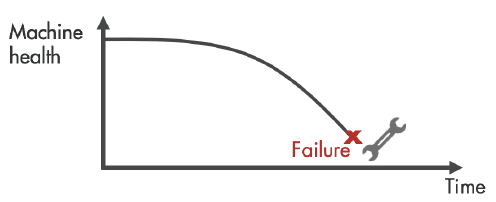
\includegraphics[width=0.45\textwidth]{Figures/Chapter03/Fig.03.01_Corrective.png}
	\caption{Corrective Maintenance (source: MathWorks)}
	\label{fig03.01}
\end{figure}

\begin{figure}[h]
	\centering
	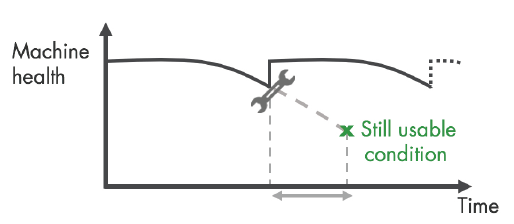
\includegraphics[width=0.5\textwidth]{Figures/Chapter03/Fig.03.02_Preventive.png}
	\caption{Preventive Maintenance (source: MathWorks)}
	\label{fig03.02}
\end{figure}

\begin{figure}[h!]
	\centering
	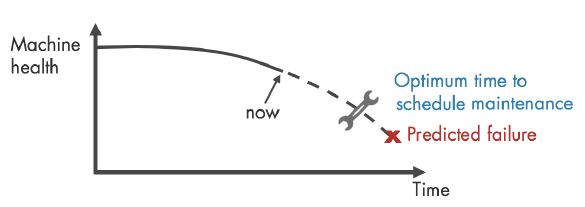
\includegraphics[width=0.6\textwidth]{Figures/Chapter03/Fig.03.03_Predictive.png}
	\caption{Predictive Maintenance (source: MathWorks)}
	\label{fig03.03}
\end{figure}

In summary, Corrective Maintenance is too late, while Preventive Maintenance can be too early. Predictive Maintenance is expected to be on time, neither early nor late. Therefore, Predictive Maintenance is the objective and also the new standard of Smart Manufacturing.


\subsection{Three levels of Predictive Maintenance}

In terms of prediction level, Predictive Maintenance can be classified to 3 levels: Anomaly Detection, Diagnosis, and Prognosis \parencite{khan2018review}.

\begin{figure}[h!]
	\centering
	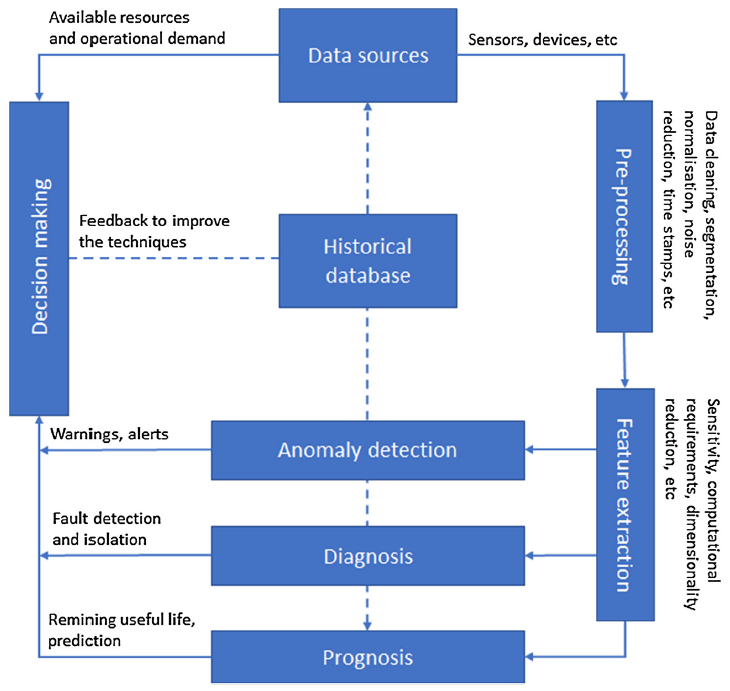
\includegraphics[width=0.6\textwidth]{Figures/Chapter03/Fig.03.04_3levels.png}
	\caption{Three levels of Predictive Maintenance \parencite{khan2018review}}
	\label{fig03.04}
\end{figure}

The first level of Predictive Maintenance is Anomaly Detection which can detect if there are anomalies. Depending on the level of anomaly, warning or alarm can be raised. The second level is Diagnosis (or Fault Identification and Isolation). This level can identify what the fault type is and where it comes from (which component in which operating cycle). The highest level of Predictive Maintenance is Prognosis. Prognosis is a process of estimation of the Remaining Useful Life (RUL) of machines in order to predict how long the machine still works in acceptable good state before maintenance must be done. Fig. \ref{fig03.05} is an illustration of these three levels.

\begin{figure}[h]
	\centering
	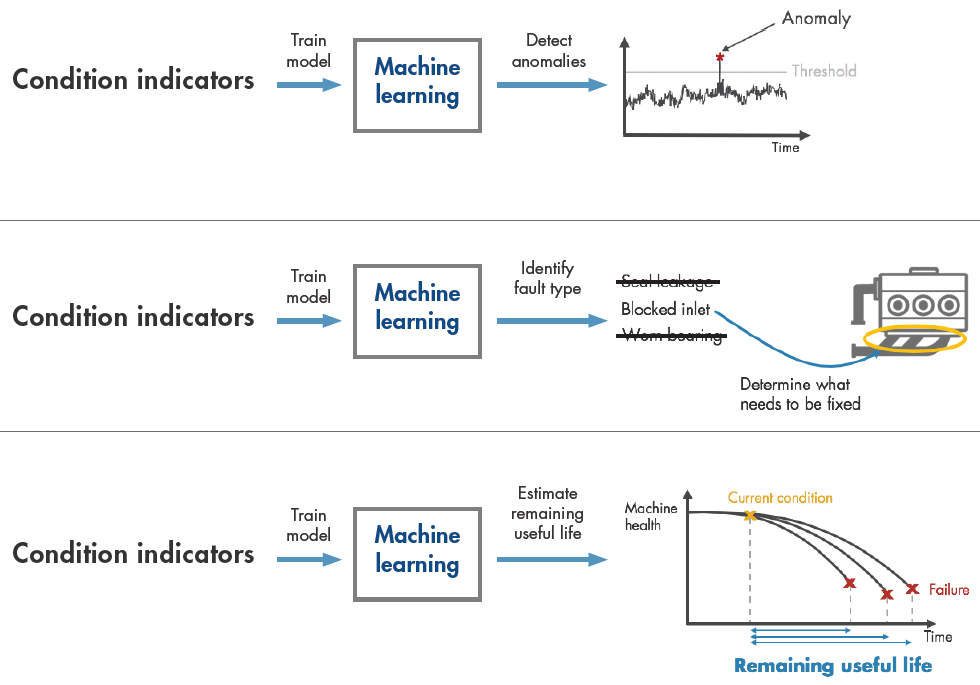
\includegraphics[width=\textwidth]{Figures/Chapter03/Fig.03.05_3_level_Matlab.png}
	\caption{Anomaly Detection, Diagnosis and Prognosis (source: MathWorks)}
	\label{fig03.05}
\end{figure}

In summary, Industrial Maintenance can be classified as Fig. \ref{fig03.06}. The level of prediction increases from left to right.

\begin{figure}[h]
	\centering
	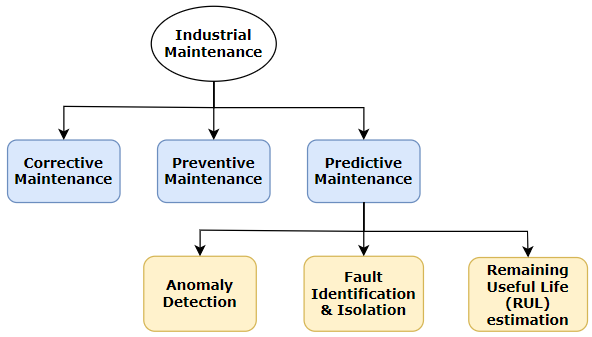
\includegraphics[width=0.75\textwidth]{Figures/Chapter03/Fig.03.06_classification.png}
	\caption{Classification of Industrial Maintenance}
	\label{fig03.06}
\end{figure}

\subsection{Industrial Machine and Machine Data}

Because the terminology Industrial Device usually refers to a tangible, stand-alone machine, in this work, the terminology “Industrial Machine” or “Machine” is used for all single industrial devices or group of related industrial devices which conduct a single or a range of industrial tasks. This terminology refers to the wide range of machines used in industrial environment from single equipment to complex machines, from traditional machines without computational capability to smart machines with embedded computer inside, from stand-alone device (e.g. fan, light…) to a group of machine working together as a compound manufacturing unit (e.g. turbine, production line, boiler system…).

In this work, the terminology “Machine Data” refers to all data related to conditions of industrial machines which can be used for Predictive Maintenance. Data can be operational data of machines or information of the machine itself (such as settings, technical specifications). Data can be measured directly or indirectly (e.g. power consumed or product rejection rate). Data can also be information of the environment where machines operate (e.g. temperature, humidity... of the industrial site).

\subsection{Data-driven approach}

Data-driven Predictive Maintenance techniques are based on data of industrial machines: historical data and new operational data. Especially, distinguishing between data of good working condition and data of failure cases is very important.

\begin{figure}[h!]
	\centering
	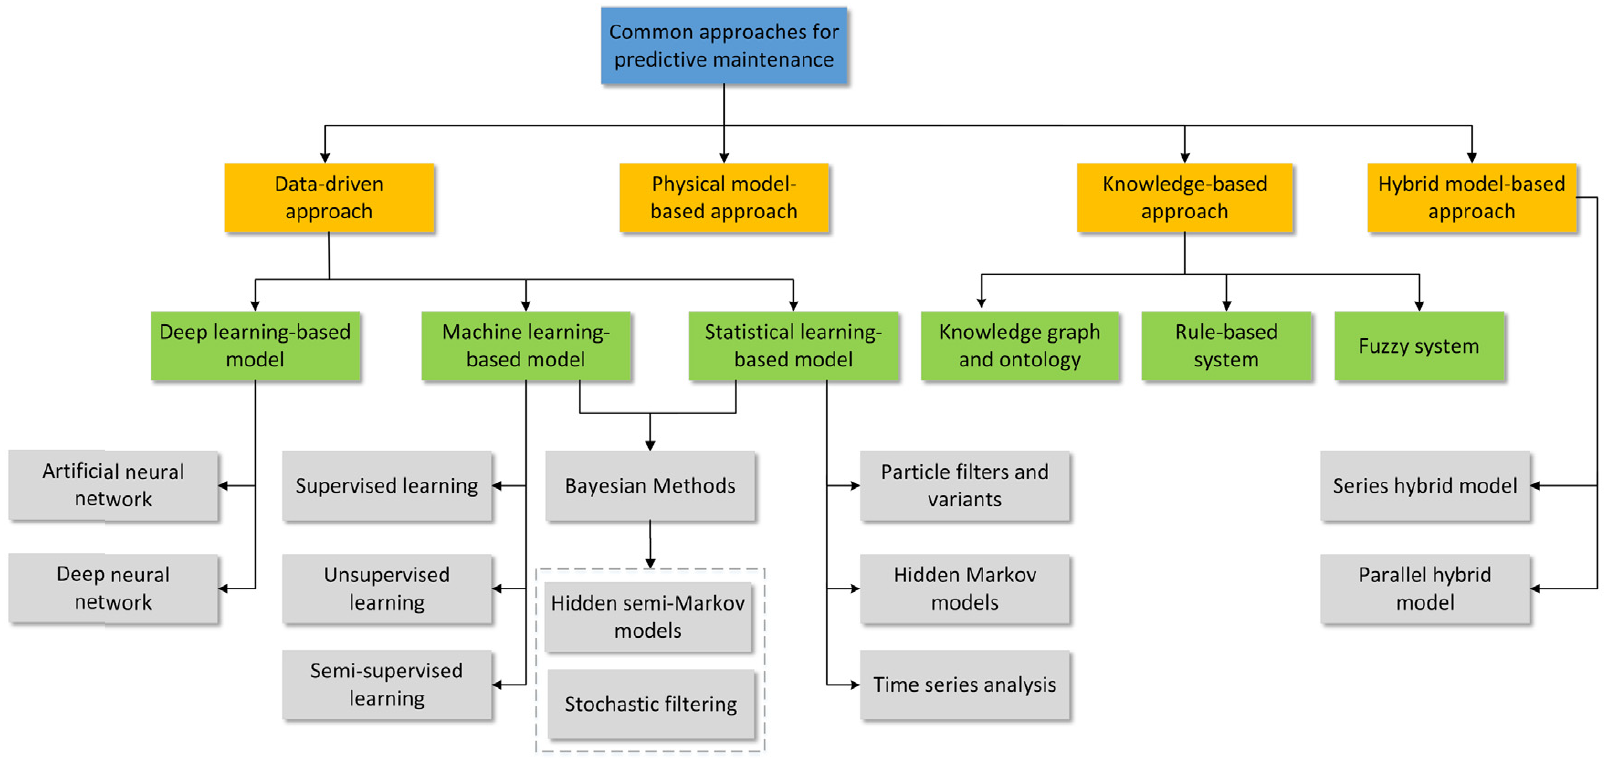
\includegraphics[width=\textwidth]{Figures/Chapter03/Fig.03.07_classification.png}
	\caption{Classification of the common predictive maintenance approaches \parencite{cao2022kspmi}}
	\label{fig03.07}
\end{figure}

Basically, Predictive Maintenance methods can be divided into the following three main categories: model-based approach, data-driven approach and knowledge-based approach (Fig. \ref{fig03.07}). The model-based approach uses a mathematical representation of the system combined with the physical understanding of industrial machines. The data-driven approach is preferred when system models are not available due to certain reasons (e.g. machine manufactures do not share or lack of expertise) but machine data is available. Knowledge-based approach implements Predictive Maintenance solution as Knowledge-based system using techniques such as knowledge graphs, ontology, rule-based or fuzzy logic. There is also the hybrid model-based approach which is a combination of model-based and data-driven approaches an attempts to leverage the strengths from both approaches \parencite{cao2022kspmi}.

Although in principle, the model-based approach can provide the most accurate diagnosis and most precise estimation of RUL, it requires a machine knowledge in very high level of detail. So except machine manufactures do it for their own machine, this approach is very difficult to implement. Similarly, knowledge-based approach need the collaboration of machine experts for building the knowledge-based system (for example: define rules).

Therefore, data-driven Predictive Maintenance has attracted wide attention in recent years, especially when industrial wireless sensor networks and industrial cyber physical systems become emerging data acquisition technologies \parencite{susto2014machine}. The increasing availability of industrial data is boosting the development and deployment of data-driven Predictive Maintenance solutions. It is believed that if we can maximize the usage of these data, we can estimate the health status of an industrial machine or even a complex industrial system, then predict when the maintenance is needed. It is also the context of this work.

In principle, any operational data related to machines can be used for Predictive Maintenance. Hashemian lists several typical type of machine data (but not limited to) which can be used as input for Predictive Maintenance \parencite{hashemian2010state}. Machine data used for Predictive Maintenance can be called Machine Condition Indicators (Fig. \ref{fig03.08}).

\begin{figure}[h!]
	\centering
	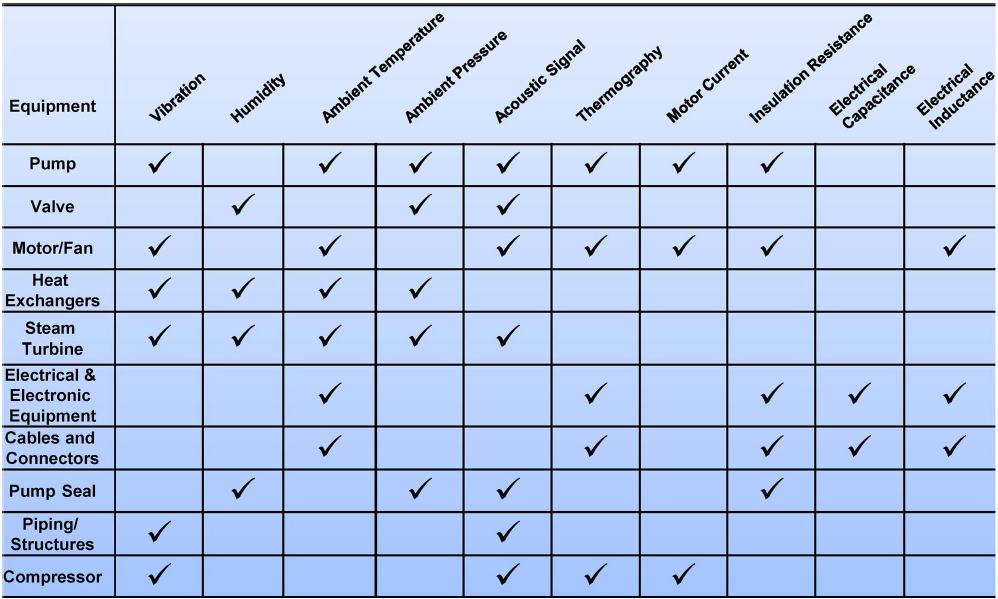
\includegraphics[width=\textwidth]{Figures/Chapter03/Fig.03.08_Indicator.png}
	\caption{Machine Condition Indicators \parencite{hashemian2010state}}
	\label{fig03.08}
\end{figure}

Data can be collected through sensors or through I/O module of machines by Programmable Logic Controller (PLC) of Supervisory Control and Data Acquisition (SCADA) systems or Industrial Distributed Control System (DCS), or machine data can be transmitted directly to data cloud in case of smart machines or smart sensors.

Besides, images (by camera, drone, satellite…) can also be used thanks to machine vision achievements, for example: photos of solar panels in solar power farm or photos of railway.

\subsection{Examples of Predictive Maintenance application}

Following are some studies of Predictive Maintenance. Only purposes of the studies are introduced. Technical aspect and performance are not presented.

\textbf{Photovoltaic panels (solar panels)}: Huuhtanen et al. apply Convolutional Neural Network (CNN) to build a regression model for detect anomalies for Photovoltaic panels of solar power plant \parencite{huuhtanen2018predictive}.

\begin{figure}[h]
	\centering
	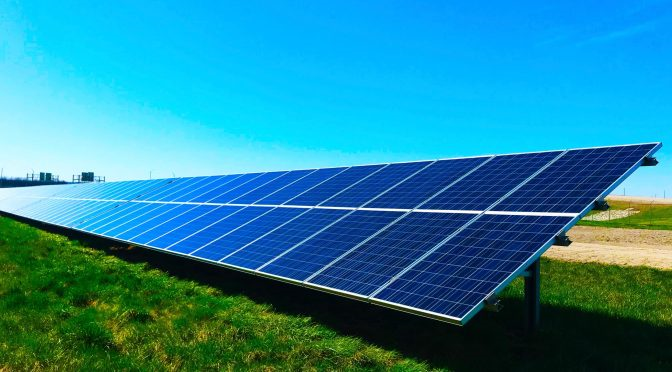
\includegraphics[width=0.6\textwidth]{Figures/Chapter03/Fig.03.09_Solar.png}
	\caption{Photovoltaic panels (source: EuroScientist. Illustration, not used in the study)}
	\label{fig03.09}
\end{figure}

Their regression models use historical data of the panel, local weather information and electricity power generated by neighboring panels in order to predict the electricity power that a panel should generate. If the predicted value is different from the real value, usually a drop of amount, there can be a probability that the panel is malfunctioning. In this case, the predictive maintenance problem is modeled as a binary classification model: “functioning” or “malfunctioning”.

\begin{figure}[h]
	\centering
	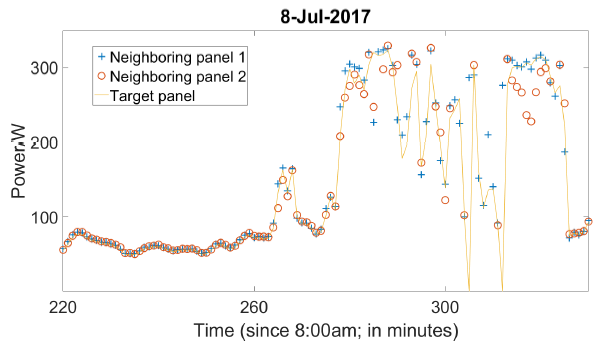
\includegraphics[width=0.8\textwidth]{Figures/Chapter03/Fig.03.10_regresssion.png}
	\caption{Regression of solar power curves  \parencite{huuhtanen2018predictive}}
	\label{fig03.10}
\end{figure}

%\hspace{1cm}\\
\textbf{Tungsten filament in semiconductor industry}: Susto et al. apply their multiple classifier approach for an industry which really needs predictive maintenance: semiconductor industry \parencite{susto2014machine}. They tested their methodology for replacing tungsten filaments used in ion implantation, one of the most important processes in semiconductor manufacturing fabrication. In Fig. \ref{fig03.11}, the filament is part of the ion source section of the tool.

\begin{figure}[h]
	\centering
	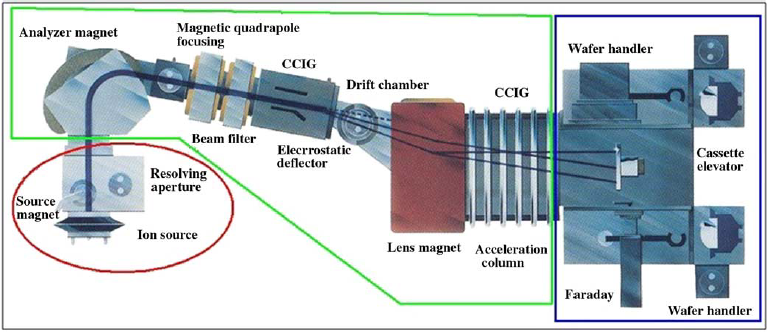
\includegraphics[width=0.9\textwidth]{Figures/Chapter03/Fig.03.11.png}
	\caption{Schematic of a generic ion implanter tool \parencite{susto2014machine}}
	\label{fig03.11}
\end{figure}

The tungsten filament is considered as a “bottleneck” in production lines due to the high cost of the tool. It must be frequently replaced. Every time a filament is changed, the tool is down for approximately 3h. 

Data used in multivariate time series data of 31 variables as following (Fig. \ref{fig03.12}).

\begin{figure}[h]
	\centering
	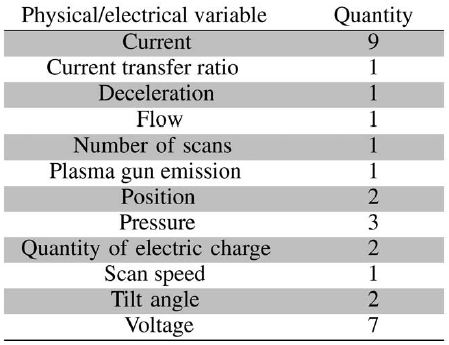
\includegraphics[width=0.5\textwidth]{Figures/Chapter03/Fig.03.12_Variable.png}
	\caption{31 physical/electrical variables \parencite{susto2014machine}}
	\label{fig03.12}
\end{figure}

They use historical data of these 31 variables to train their multi-class classification model. Then the trained model is used to predict new data in order to classifier the degradation level of this component. Because the existing maintenance policy is Run-to-Failure (R2F), there are enough failure data for training the multiple classification model.


\section{Deep Learning for the Predictive Maintenance problem}

The core of the data-driven Predictive Maintenance system are Predictive models. Historical data of the industrial machines are used to build or to train predictive models. Then new operational data will be used to detect anomalies, identify faults and estimate Remaining Useful Life (RUL) of machines in order to predict when maintenance are needed.

Predictive Maintenance problems can be modeled using any Machine Learning technique \parencite{khan2018review}. However, Deep Learning is widely used in more and more researches. In this work, Deep Learning is also adopted. The reason why Deep Learning is preferred is presented below.

\subsection{Concept of Deep Learning}

In data-driven approach, two popular methods are learning-based method and statistical-based method. Learning-based method utilizes Machine Learning techniques while statistical-based method is based on statistical models. Although many machine learning techniques are theoretically based on statistical theory, they are usually classified as two different methods \parencite{cao2022kspmi}.

Machine Learning, a branch of AI, refers to techniques which have the ability to acquire their own knowledge, by extracting patterns from raw data (or from experience) without being explicitly programmed. Deep Learning is a branch of Machine Learning based on Neural Network.

\begin{figure}[h]
	\centering
	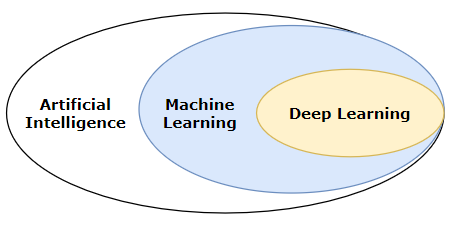
\includegraphics[width=0.55\textwidth]{Figures/Chapter03/Fig.03.13_DL.png}
	\caption{AI, Machine Learning and Deep Learning}
	\label{fig03.13}
\end{figure}

For reference, below is the clarification of these concepts by Microsoft \parencite{microsoft-dl}.

\textbf{Artificial Intelligence (AI)} is a technique that enables computers to mimic human intelligence. It includes machine learning.

\textbf{Machine Learning} is a subset of artificial intelligence that uses techniques (such as deep learning) that enable machines to use experience to improve at tasks.

\textbf{Deep Learning} is a subset of machine learning that's based on artificial neural networks that permit a machine to train itself to perform a task. The learning process is deep because the structure of artificial neural networks consists of multiple input, output, and hidden layers. Each layer contains units that transform the input data into information that the next layer can use for a certain predictive task. Thanks to this structure, a machine can learn through its own data processing.

Basically, Deep Learning are machine learning models which are variations of Neural Network. The origin of the name “Deep Learning” is because neural networks used in Deep Learning usually have multiple hidden layers. Fundamental concepts of Deep Learning is presented in \ref{part3.2.3}.

In terms of implementation, most of traditional Machine Learning are algorithms (e.g. such as Decision Tree, Support Vector Machine, Isolation Forest…). Nowadays, the terminology Machine Learning is often used for all Machine Learning techniques which are not Deep Learning.

\subsection{Supervised, Unsupervised and Semi-Supervised Learning}

In terms of learning type, both traditional Machine Learning and Deep Learning can be divided into two main groups: Supervised Learning and Unsupervised Learning (Fig. \ref{fig03.14}). This classification is based on the fact that the dataset used for training the model is labeled or unlabeled. 

\begin{figure}[h]
	\centering
	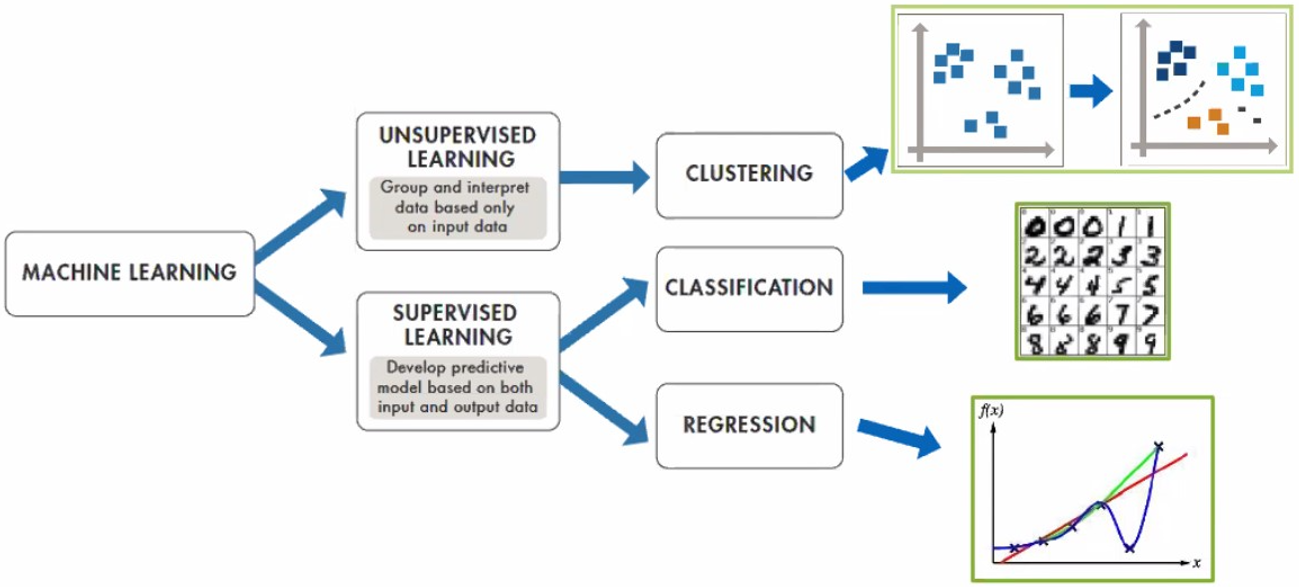
\includegraphics[width=\textwidth]{Figures/Chapter03/Fig.03.14_Learning_Type.png}
	\caption{Supervised and Unsupervised Learnings (source: MathWorks)}
	\label{fig03.14}
\end{figure}

Classification problem is the task of identifying which group the data belong to. Typical example is image recognition (e.g. flower, fruit, vegetable, animal, vehicle, human face… or object type in general). 

Regression problem is the task of prediction of a continuous value (e.g. temperature of climate, fuel consumption of cars, water level of rivers or price of house that clients accept to buy…).

Clustering problem is the task of grouping data based on criteria of similarity. The number of group can be predefined or also discovered by the learning process. Similarly, criteria for grouping can be predefined or can also be discovered during the learning process.

Due to the nature of these problems, classification and regression problems need labelled data while clustering problems can work with unlabeled. In labeled data, the expected result (the label) is known while unlabeled data are just raw data.

Semi-Supervised Learning is the hybrid type between supervised learning and unsupervised learning. This approach combines the majority of unlabeled data with few labeled data. Semi-Supervised Learning has important role in the proposed solution of this work and will be presented in details in \ref{part3.3}.

Besides, a special branch of Machine Learning is Reinforcement Learning (RL). RL uses the trial-and-error strategy and improves by evaluating the reward (what is the reward and how to evaluate reward depend on the problem). Reinforcement Learning is useful for applications such as Intelligent Agent. Reinforcement Learning can be implemented by Estimated Value Functions or Genetic Algorithms. However, Reinforcement Learning is not considered in this work.


\subsection{Fundamental concepts of Deep Learning} \label{part3.2.3}

\textbf{Perceptron (artificial neuron)}: Be inspired by the human neural, the simplest unit of neural networks is the Perceptron (Fig. \ref{fig03.15}).

\begin{figure}[h]
	\centering
	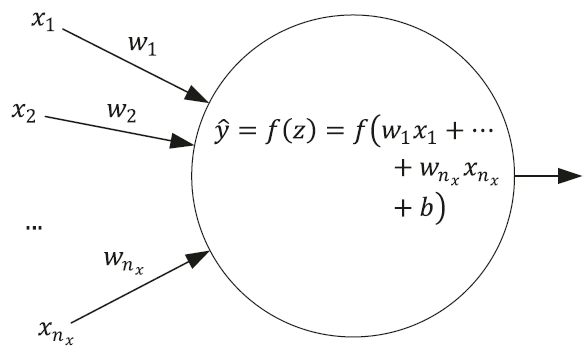
\includegraphics[width=0.55\textwidth]{Figures/Chapter03/Fig.03.15_perceptron.png}
	\caption{A perceptron \parencite{michelucci2018applied}}
	\label{fig03.15}
\end{figure}

% https://www.overleaf.com/learn/latex/Subscripts_and_superscripts#Operators_using_subscripts_and_superscripts
Mathematical formula of a perceptron is: 
\begin{center}
	\[ y = f(z) = f(\sum_{i=1}^{n} {w_{i}x_{i}} + b) \]
\end{center}

Output of an artificial neuron depends on: 

- inputs from previous layer $x_{1}$, $x_{2}$, ..., $x_{n}$ (and also recurrent feedback from next layer in case of Recurrent Neural Network)

- weights of each inputs $w_{1}$, $w_{2}$, ..., $w_{n}$

- activation function \textbf{f}. All neurons of a layer have the same activation function. Therefore, activation function is also called Layer Activation Function.

- There is also \textbf{b} which stands for “bias”. Bias is optional because it is actually an adjustment parameter.

\textbf{Multi-Layer Perceptron (MLP)} is the basic Neural Network architecture (Fig. \ref{fig03.16}). It is built by stacking layers of perceptron. MLP consists of at least three layers: an input layer, a hidden layer, and an output layer. MLP is fully connected, because each perceptron receives input from each perceptron in the previous layer and feeds its output to every perceptron in the next layer. Each input will be multiplied with a weight \textbf{w}. All of these weights $w_{i,j}$ are trainable parameters of the neural network.

\begin{figure}[h]
	\centering
	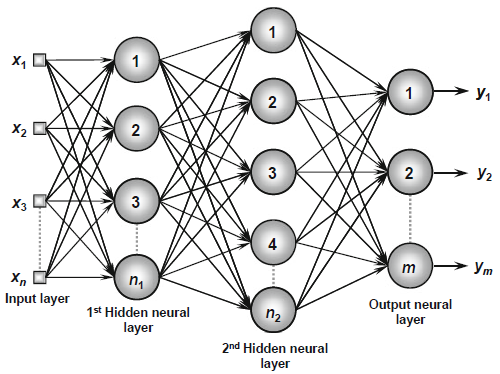
\includegraphics[width=0.65\textwidth]{Figures/Chapter03/Fig.03.16_MLP.png}
	\caption{Multi-Layer Perceptron \parencite{da2017artificial}}
	\label{fig03.16}
\end{figure}

MLP is also called Feed Forward Neural Network (FFNN) because output of a perceptron is only sent to next layer and is never be sent back to the previous layer (unlike Recurrent Neural Network architecture, Fig. \ref{fig03.17}). Sometimes the terminology Artificial Neural Network (ANN) is used to refer to FFNN.

\textbf{Recurrent Neural Network (RNN)} is a neural network architecture in which output of a perceptron can be shared back to previous layers (Fig. \ref{fig03.17}). This architecture is needed for processing of sequential data such as language translation, or stock market prediction.

\begin{figure}[h]
	\centering
	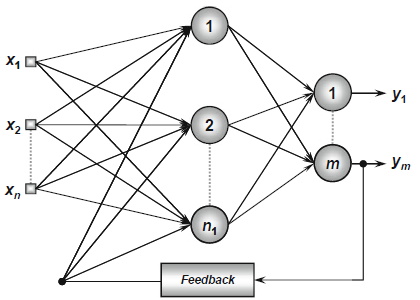
\includegraphics[width=0.5\textwidth]{Figures/Chapter03/Fig.03.17_RNN.png}
	\caption{Recurrent Neural Network \parencite{da2017artificial}}
	\label{fig03.17}
\end{figure}

\textbf{Convolution Neural Network (CNN)} is a variation of Feed Forward Neural Network which is very strong in feature extraction. It has two special operations, convolution operation and pooling operation, for extracting features. Although it is originally created for image classification, now it has applications in many other fields including Predictive Maintenance. It will be used in implementation of Deep Learning architectures that need strong feature extraction ability, in case the standard FFNN is not enough powerful.

\textbf{Generative Adversarial Network (GAN)} are Deep Learning architectures that can generate new content based on existing content. A famous application of GAN is DeepFake.

\textbf{AutoEncoder (AE)} is Feed Forward Neural Network type which can reconstruct the input data. AutoEncoder has an important role in proposed solution of this work. Details of AutoEncoder will be presented in this chapter.

\textbf{Activation function} of each neuron is the function f to convert the real weighted input vector to a real value: 
%\[ y = f(z) = f(\sum{w_{i}x_{i}}), i=1..n \]
\[ y = f(z) = f(\sum_{i=1}^{n} {w_{i}x_{i}}) \]
%y = f(z) with z = sum(wixi).
Which activation function is selected depends on the problem that needs to be modeled. For example, with unit step activation function, the Neural Network will become a one-class classifier.

\textbf{\textit{Unit step}} activation function is the simplest activation function (Fig. \ref{fig03.18}). It is also called binary step, threshold or ladder activation function. The threshold can be different from 0 if the bias is added to the neural network.

\begin{figure}[h]
	\centering
	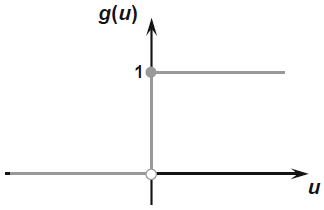
\includegraphics[width=0.35\textwidth]{Figures/Chapter03/Fig.03.18_unit.png}
	\caption{Unit step activation function \parencite{da2017artificial}}
	\label{fig03.18}
\end{figure}

\textbf{\textit{Identity (Linear)}} activation function is also a basic activation function with the formula g(u) = u (Fig. \ref{fig03.19}).

\begin{figure}[h]
	\centering
	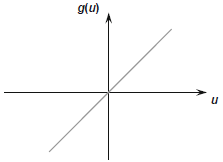
\includegraphics[width=0.35\textwidth]{Figures/Chapter03/Fig.03.19_Linear.png}
	\caption{Linear activation function \parencite{da2017artificial}}
	\label{fig03.19}
\end{figure}

Below are popular activation functions used in most of Deep Learning models.

\textbf{\textit{Rectified Linear Unit (ReLU)}} activation function has output value from 0 to 1 with the following formula f(z) = max(0, z). \textbf{\textit{Leaky ReLU}} activation function is a variation of ReLU of which the output value can be smaller than 0.

\begin{figure}[h!]
	\centering
	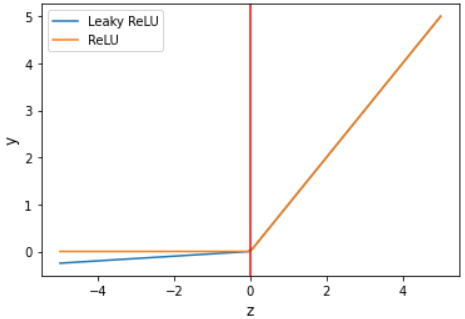
\includegraphics[width=0.6\textwidth]{Figures/Chapter03/Fig.03.20_ReLU.png}
	\caption{ReLU and Leaky ReLU activation functions}
	\label{fig03.20}
\end{figure}

\textbf{Sigmoid} activation function has output value from 0 to 1. \textbf{Tanh (Hyperbolic Tangent Activation)} activation function has output value from -1 to 1. They are nonlinear activation functions (Fig. \ref{fig03.21}).

\begin{figure}[h!]
	\centering
	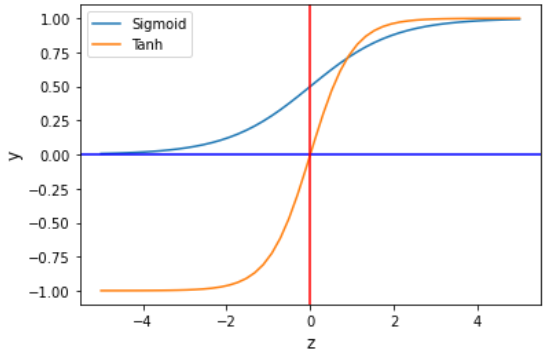
\includegraphics[width=0.5\textwidth]{Figures/Chapter03/Fig.03.21_Sigmoid.png}
	\caption{Sigmoid and Tanh activation functions}
	\label{fig03.21}
\end{figure}

Besides, there are also specific activation functions which can be used for special purposes by advanced experts, for example: Gaussian activation function (Fig. \ref{fig03.22}).

\begin{figure}[h]
	\centering
	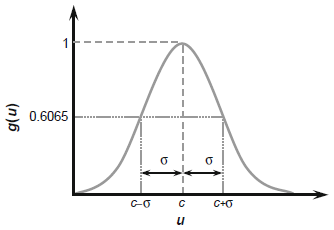
\includegraphics[width=0.5\textwidth]{Figures/Chapter03/Fig.03.22_Gaussian.png}
	\caption{Gaussian activation function}
	\label{fig03.22}
\end{figure}

\textbf{\textit{Softmax activation function for classification}}: Softmax activation function is a special activation function used for the last layer of classification models.

The Classification model has to capture an underlying function y = f(x) from the training dataset in which:

x = ($x_{1}$, $x_{2}$,..., $x_{n}$) is input data.  Input can be a multivariate data sample or a data frame (a sequence of data sample).

y = ($y_{1}$, $y_{2}$,..., $y_{m}$) is output. They are probabilities that the input belongs to each classified class. 

So sum of outputs of the last layer must be 100\%.
%\begin{center}
\[ y_{1} + y_{2} + y_{3} + ... + y_{m} = 1 \]
%\end{center}

Therefore, regardless the implementation of input layer and hidden layers, the last of the Classification model often:

- is fully connected with the previous layer. Each neuron receives inputs from al neurons of the previous layer.

- has softmax activation function which converts a vector of values to a probability distribution

Softmax activation function converts a real vector to a vector of categorical probabilities. The elements of the output vector are in range (0, 1) and sum to 1. Softmax is often used as the activation function for the last layer of a classification network because its special characteristic can be used to represent the probability distribution  (\url{https://keras.io/api/layers/activations/}).

%https://www.overleaf.com/learn/latex/Integrals%2C_sums_and_limits#Sums_and_products

The formula of Softmax activation function ensures that total distribution of all probabilities is 100\% \parencite{michelucci2018applied}.
\[
S(z)_{i} = \frac { e^{z_{i}} } { \sum_{j=1}^{k} e^{z_{j} } }
\]
%\[ \sum_{j=1}^{k} e^{z_{j}} \]

%Fig. 3.22. Softmax activation fuction \parencite{michelucci2018applied}
%This formula ensures that total distribution of all probabilities is 100%.
%Fig. 3.23. Probability distribution \parencite{michelucci2018applied}

\textbf{Training the Neural Network} is a process of adjusting all weights $w_{i,j}$ of all perceptrons of all layers so that output of the last layer is as close as possible to expected output.

This objective can be done thanks to Backward Propagation algorithms implemented in any Deep Learning programming framework. Most of Backward Propagation algorithms are based on Gradient Descent algorithm, an iterative optimization algorithm.

During the training process, for each sample batch of training data, the computation includes

- Calculate the output

- Calculate the distance between the output and the expected result

- Run a Backward Propagation algorithm to adjust all trainable parameters so that the output will be a bit closer to the expected result

These steps will be repeated until the whole training dataset is processed. One time that the whole dataset is processed is called an \textbf{epoch}. The number of epoch of the training process can be hundred or even thousand.

The number of epoch increases until the accuracy cannot be improved. It means the training process is converged and this state is called the convergence.

Training Neural Network is a very heavy process. Let’s examine a simple Deep Learning model for classification of animal images. This is a standard FFNN with input as 200x200 pixel images (reshaped as one-dimension array of 40,000 real numbers) and output are 100 animal types. It has 5 hidden layers, each layer has 64 perceptrons. This model has up to 2,5 million trainable parameters (Fig. \ref{fig03.23}).

\begin{figure}[h]
	\centering
	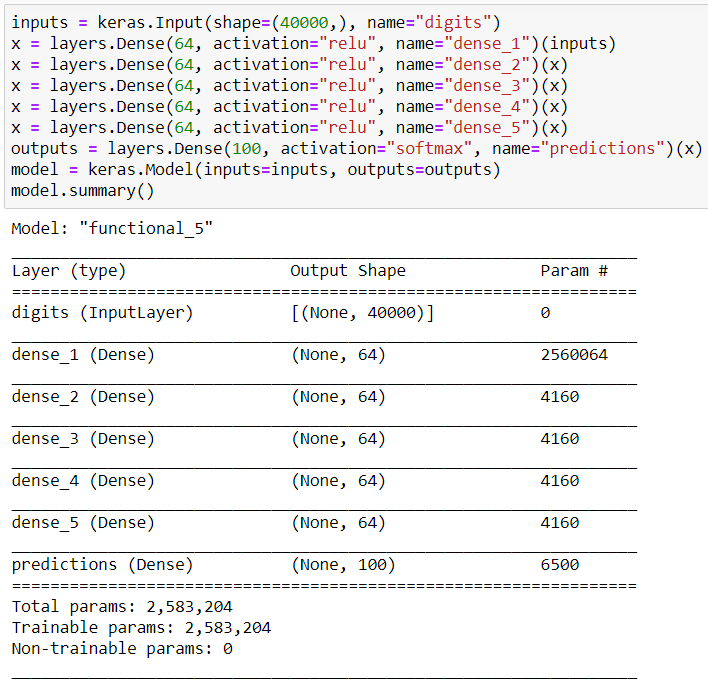
\includegraphics[width=0.9\textwidth]{Figures/Chapter03/Fig.03.23_FFNN.png}
	\caption{A Feed Forward Neural Network structure and parameters}
	\label{fig03.23}
\end{figure}

If the training dataset contains 10,000 images and the model needs to be trained 100 (can be more) cycles (epochs) before being converged, it takes much time and computational resource. Moreover, this is standard Neural Network without recursive mechanism. With more complicated models such as Long Short-Term Memory (LSTM), the computation is much heavier.

Training the Neural Network is all called the \textbf{fitting} process, because it makes the model fitted in the training dataset. Once a model is fitted with the training dataset, this model can predict well all data sample of this dataset. Usually the accuracy need to be at least 90\% so that it can be deployed to production.

\textbf{Hyperparameter}: During the training process, many other parameters need to be set such as number of epoch, batch size, optimization algorithm, loss function… These parameters don’t belong to the neural network but are used to control the training process. They are called hyperparameter. The process of selecting the best combination of hyperparameters for training is called hyperparameter turning.

\textbf{Prediction}: Once the model is trained, it can be used for prediction. Prediction of a data sample is to pass this data sample as input of first layer of the model and to receive the output from the last layer of the model. Depending on the model, the prediction output will be a single value or an array of value. Prediction can be done for a single data input or a whole input dataset at the same time. Prediction result of a whole dataset, which is an array of data sample, will be simply an array of prediction output.

Although training the neural network is heavy, using the trained model for prediction is quite fast. Prediction process is as fast as calling a numerical function with a chain of simple numerical and logical operations thanks to the structure of the MLP. All computation is calculated in memory and inside of the Neural Network. CNN and LSTM are more complicated, but still fast enough for systems that need to provide quick response.

\textbf{Generalization}: A good generalization is the objective when building a Deep Learning model. A Deep Learning model generalizes well a problem (or a real system) if it  not only predicts correctly the training dataset but also predicts well new data.

\textbf{Underfitting and Overfitting}: If the model cannot generalize well the problem (or the real system), it can fall into underfitting or overfitting case. Underfitting is the case that the training process cannot be converged with the training dataset. Overfitting is the case that the model predicts too perfectly with the training dataset but works badly with new data. There are many specific ways and techniques to overcome these two challenges.

\begin{figure}[h]
	\centering
	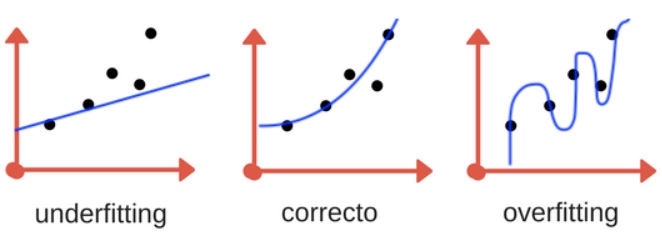
\includegraphics[width=0.6\textwidth]{Figures/Chapter03/Fig.03.24_Overfitting.png}
	\caption{Underfitting versus Overfitting (source: aprendemachinelearning.com}
	\label{fig03.24}
\end{figure}

\subsection{Why Deep Learning is preferred for Predictive Maintenance?}

The core of the data-driven Predictive Maintenance system are Prediction models which are trained by historical data of industrial machines and then can predict necessary maintenance. In principle, any Machine Learning technique can be used to implement these predictive models. However, Deep Learning is preferred research in recent years.

Compared to traditional Machine Learning algorithms, Deep Learning models require more data, computational resource and time to train but requires less domain knowledge (Fig. \ref{fig03.25}).

%Zhang et al. compare the flows of applying Traditional Machine Learning and Deep Learning for Predictive Maintenance and explain why Deep Learning is more adopted \parencite{zhang2019data}. The reason is Deep Learning can avoid complex feature engineering steps that need domain knowledge of machine and process. In Fig. 74, we can see that traditional Machine Learning is a bit like the hybrid approach between model-based approach and data-driven approach. It is more suitable for specific, critical and expensive industrial systems than for building a general and scalable Predictive Maintenance solution. Instead, Deep Learning moves directly to an end-to-end learning.

\begin{figure}[h]
	\centering
	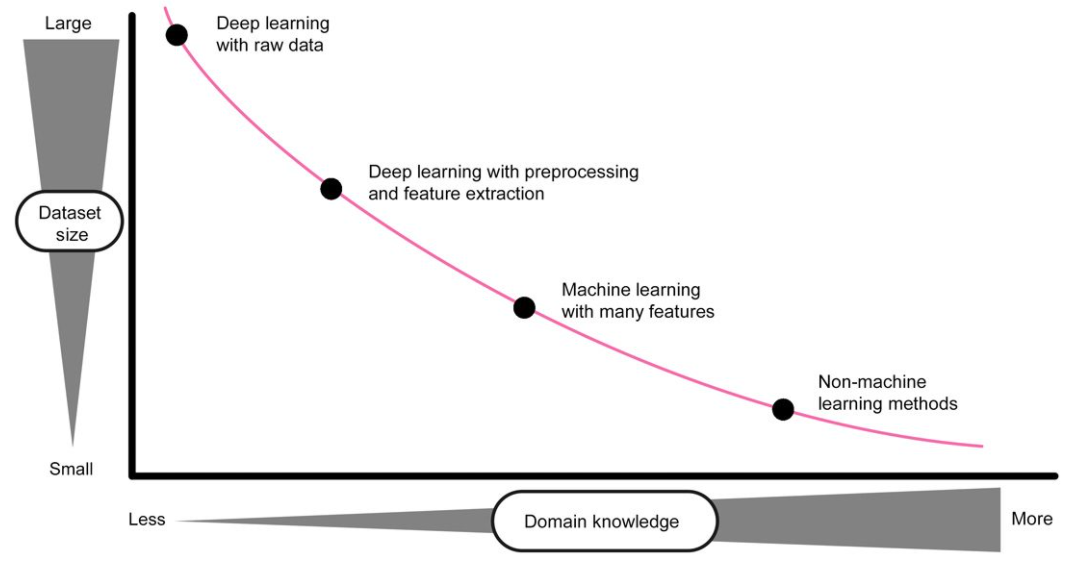
\includegraphics[width=\textwidth]{Figures/Chapter03/Fig.03.25_DL_ML.png}
	\caption{Deep Learning versus Machine Learning (\url{https://es.mathworks.com/campaigns/offers/next/practical-guide-to-deep-learning/collecting-data.html})}
	\label{fig03.25}
\end{figure}

The performance of Deep Learning relies heavily on the training data. However, with the development of IIoT, big industrial dataset for Deep Leaning is no longer rare, although there are still challenge with data quality and data fusion.

Zhang et al. compare the flows of applying Traditional Machine Learning and Deep Learning for Predictive Maintenance and explain why Deep Learning is more adopted \parencite{zhang2019data}. The reason is Deep Learning can avoid complex feature engineering steps that need domain knowledge of machine and process. In Fig. \ref{fig03.26}, we can see that traditional Machine Learning is a bit like the hybrid approach between model-based approach and data-driven approach. It is more suitable for specific, critical and expensive industrial systems than for building a general and scalable Predictive Maintenance solution. Instead, Deep Learning moves directly to an end-to-end learning.

\begin{figure}[h]
	\centering
	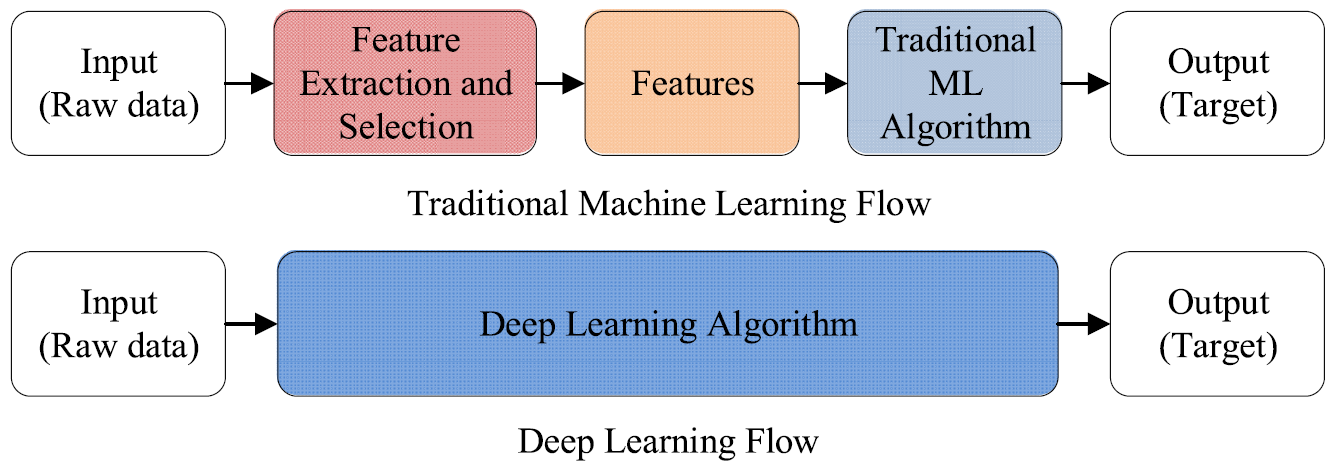
\includegraphics[width=0.95\textwidth]{Figures/Chapter03/Fig.03.26_DL_ML.png}
	\caption{Machine Learning and Deep Learning flows}
	\label{fig03.26}
\end{figure}

Olga Fink also analyzes reasons why Predictive Maintenance solutions need to change from feature engineering to feature learning due to the large number of different types of sensors, resulting a very heterogeneous condition monitoring data. Traditional machine learning which requires manual feature engineering steps show many limitations such as limited scalability or dependence on domain experts. End-to-end learning architectures of deep learning allows to use directly raw data input, with automatic feature learning steps within the neural network architectures \parencite{fink2020data}.

Deep Learning is more suitable for building a general and scalable Predictive Maintenance solution which is the ambition of the research community. This is the reason why Deep Learning is chosen in this work.

\textbf{Conclusion}: In order to model a problem or a physical system using Deep Learning for a certain purpose, including Predictive Maintenance, it is necessary to:

\begin{itemize}
	\item Choose or create the suitable Deep Learning model structure
	\item Have to good training dataset
	\item Build an effective training process
\end{itemize}
%- Choose or create the suitable Deep Learning model structure
%- Have to good training dataset
%- Build an effective training process

\begin{figure}[h]
	\centering
	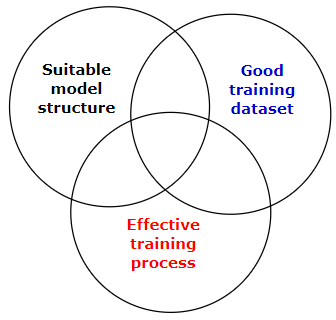
\includegraphics[width=0.4\textwidth]{Figures/Chapter03/Fig.03.27.png}
	\caption{Conditions for of Deep Learning approach}
	\label{fig03.27}
\end{figure}

Selection of the suitable model structure means to decide which is the best way to model the problem (classification, regression, clustering, generative, autoencoder…) then decide which basic Deep Leaning model (FFNN, CNN, LSTM…) should be used to implement the designed model. After that, how many layers, size of each layer, activation function for each layer… also need to be optimized.

A good training dataset is not only big enough but also represents well the problem (or the real physical system). Requirements for a good training dataset depends on the selected model and vice versa, selection of model must refer to available training data.

Finally, effective training process is crucial for having a useful model, including not only hyperparameter turning but also data preprocessing. Deep Learning models not only needs to be trained one time but also need be re-trained periodically. Otherwise, the model will be drifted (obsolete) due to lack of training with recent data.

Although Deep Learning has an important role in the proposed solution of this work, the primary topic of this TMF is not Machine Learning nor Data Science. Therefore, in this work, we will not try to explain, improve or invent new Deep Learning models. Instead, we utilise Deep Learning models justified by state-of-the-art studies and follow best practices recommended by research community and professional experts.

\section{Semi-Supervised Learning for Anomaly Detection} \label{part3.3}

\subsection{Supervised learning methods for Predictive Maintenance}

Although supervised learning approach is not chosen in this work, some studies of Predictive Maintenance using supervised learning method are briefly presented, in order to understand why supervised learning is not always applicable in real life.

In the predictive maintenance flow proposed by Rivas et al., there are two steps \parencite{rivas2019predictive}. First, a binary classification model classifies if the operating cycle before failure of the machine is bigger or smaller than 100. If the number of machine cycle before failure is smaller than 100, in the second step, a regression model will estimate RUL by predicting the concrete number of cycle. Both classification and regression models are implemented by LSTM (Fig. \ref{fig03.28}). Dataset C-MAPSS, a Run-to-Failure experimental dataset, is used to testing \parencite{saxena2008turbofan}. In the C-MAPSS dataset, the label is the number of cycle before the engine crashes.

\begin{figure}[h]
	\centering
	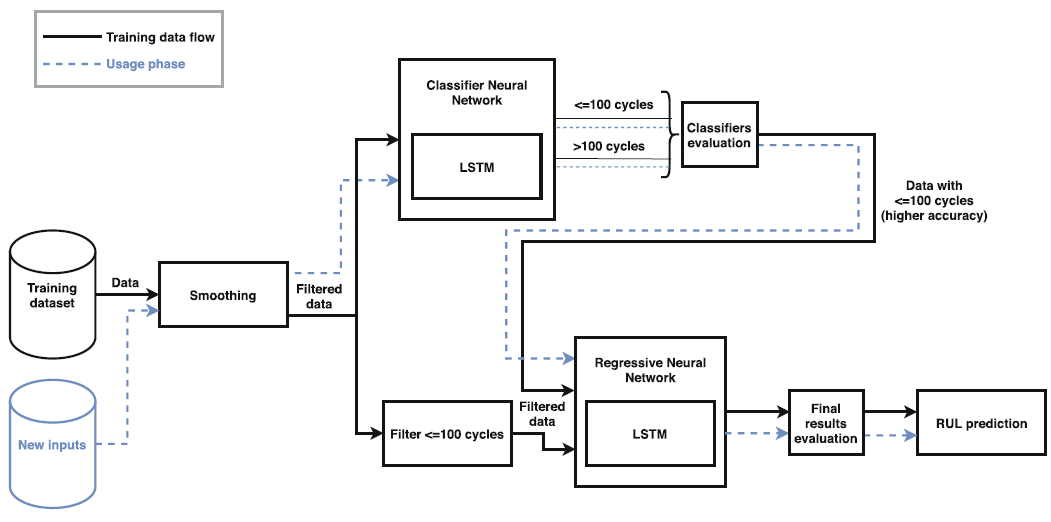
\includegraphics[width=\textwidth]{Figures/Chapter03/Fig.03.28.png}
	\caption{Classification and Regression models implemented by LSTM \parencite{rivas2019predictive}}
	\label{fig03.28}
\end{figure}

Meesublak et al. uses one-dimension Convolutional Neural Network (1D CNN) to classify conditions of bearing \parencite{meesublak2020cyber}. Bearing is the key components of rotating machinery (Fig. \ref{fig03.29}).

\begin{figure}[h]
	\centering
	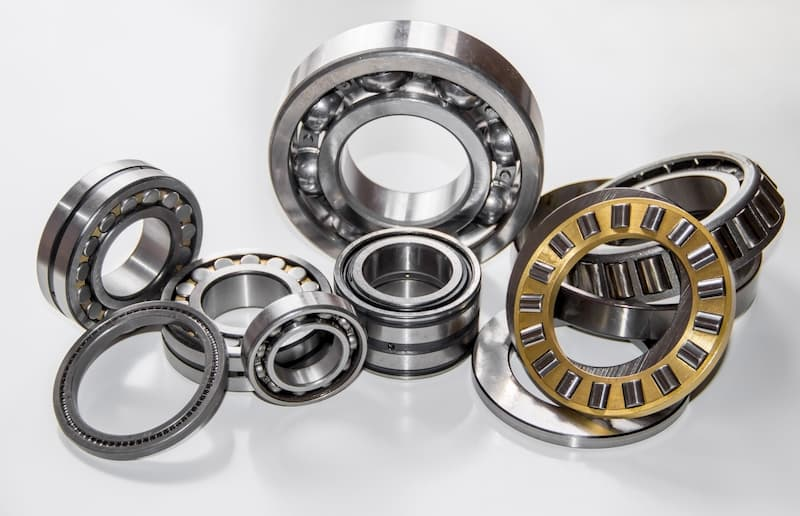
\includegraphics[width=0.35\textwidth]{Figures/Chapter03/Fig.03.29_Bearing.png}
	\caption{Ball bearing (source: Fractory. Illustration, not used in the study)}
	\label{fig03.29}
\end{figure}

1-D CNN is a simplified version of the standard two-dimension CNN (2-D CNN) created for image classification (Fig. \ref{fig03.30}). Input is 1-dimension array of univariate vibration signal.

\begin{figure}[h]
	\centering
	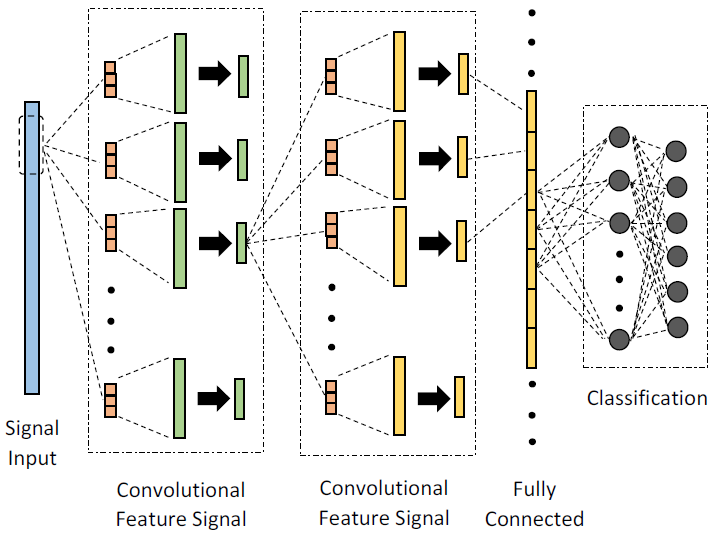
\includegraphics[width=0.7\textwidth]{Figures/Chapter03/Fig.03.30.png}
	\caption{Classification model implemented by CNN \parencite{meesublak2020cyber}}
	\label{fig03.30}
\end{figure}

Dataset used for testing is the bearing vibration data collected by the Bearing Data Center at Case Western Reserve University. The vibration signal data were monitored in at the frequency of 12,000 samples per second. Output of the model are labels as Fig. \ref{fig03.31}.

\begin{figure}[h!]
	\centering
	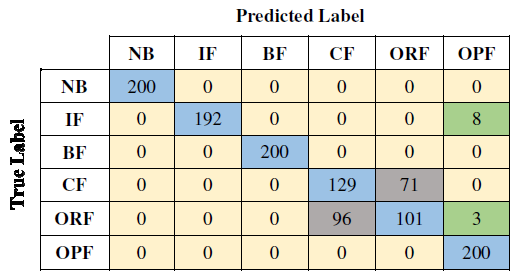
\includegraphics[width=0.5\textwidth]{Figures/Chapter03/Fig.03.31.png}
	\caption{Bearing condition classification \parencite{meesublak2020cyber}}
	\label{fig03.31}
\end{figure}

Six labels are categorical conditions of bearing: Normal Baseline (NB), Inner Race Fault (IF), Ball Fault (BF), Outer Race Centered Fault (CF), Outer Race Orthogonal Fault (ORF), and Outer Race Opposite Fault (OPF). Because bearing is quite standardized component (it has the same design principle in any machine), it is expected that the trained model can be used for real cases.

\subsection{The need of Semi-Supervised learning}

Although Classification and Regression models can produce very positive results, we can see that very few supervised learning studies can be tested with real life case studies because these models need to be trained by labelled dataset. Especially, the dataset also needs to be balanced with 20\%-30\% (or at least 5\%-10\%) data of failures. The real balanced dataset like that is very rare in industrial environment because very few (or even zero) failures is the objective of industrial management.

Therefore, most of studies using Supervised Learning approach have to use experimental datasets to verify their Deep Learning models. For example, Meesublak et al. use vibration signal of bearing in database collected by the Bearing Data Center at Case Western Reserve University \parencite{meesublak2020cyber}. Especially, many studies develop their models using the C-MAPSS dataset which is a Run-to-Failure experimental dataset shared by NASA \parencite{saxena2008turbofan}. To create this dataset, NASA runs aircraft engines from new condition until they crash. During this progress, vibration signals are measured and the number of cycle before failures is used as data label.

We never have much failure data in real world because machine failure is rare event in nature. Sometimes it does not exist, especially with new industrial systems, and when it happens, label is often inconsistent or ambiguous \parencite{serradilla2021adaptable}. For example, below is real failure information of a wind power plant during the year 2016.

\begin{figure}[h]
	\centering
	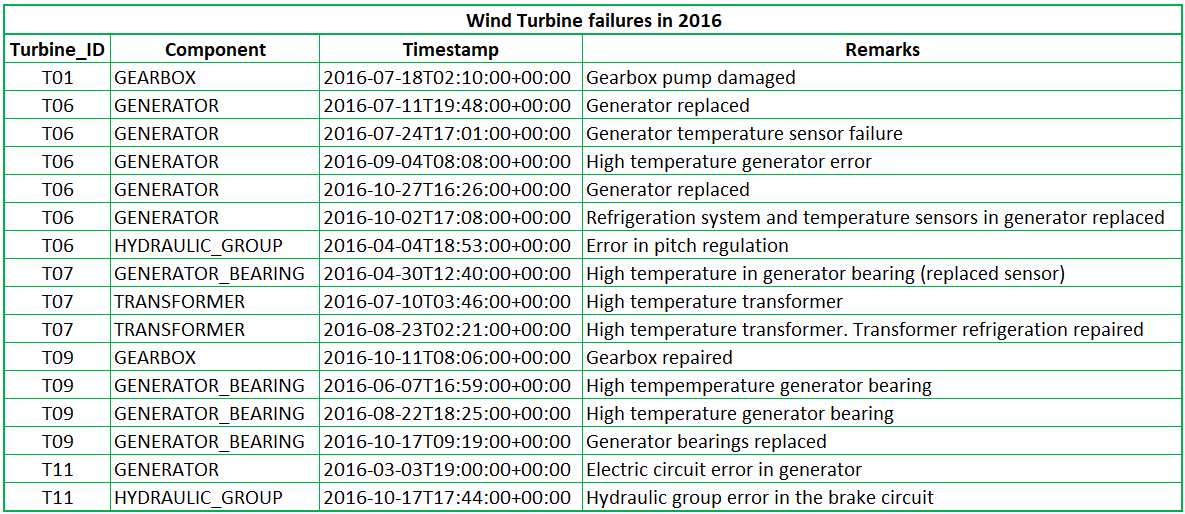
\includegraphics[width=\textwidth]{Figures/Chapter03/Fig.03.32.png}
	\caption{Wind Turbine failure information \parencite{edp18}}
	\label{fig03.32}
\end{figure}

We can see that failures are not only rare but also poor described without error classification, severity level, duration of downtime, or clear border between good and failure statuses...

By all of above reasons, studies on semi-supervised learning approach for the Predictive Maintenance problem are increasing in recent years. Semi-supervised learning is an machine learning approach that needs only a small amount of labeled data combining with a large amount of unlabeled data for training the models. Labeled data can be real or simulated data for verifying the trained models.


\subsection{Semi-supervised Anomaly Detection}

Most of solutions for Fault Classification (Diagnosis) and RUL (Prognosis) problems are supervised learning models which need labelled and balanced data for training. Unsupervised learning methods for these problems is very rare.

\begin{figure}[h]
	\centering
	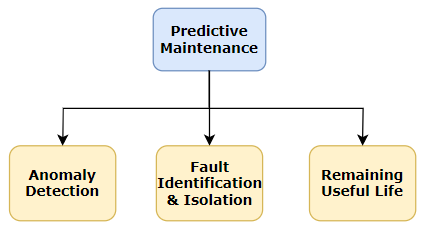
\includegraphics[width=0.55\textwidth]{Figures/Chapter03/Fig.03.33.png}
	\caption{Three levels of Predictive Maintenance}
	\label{fig03.33}
\end{figure}

However, for the first level of Predictive Maintenance which is Anomaly Detection (or Outlier Detection) (Fig. \ref{fig03.34}), the unsupervised learning approach is more popular. Anomaly detected can be point anomaly or pattern anomaly. Anomaly detection methods can vary from simple thresholds of single signal to statistics, machine learning or deep learning models. For example, Zhao et al. use Correlation-Based method for anomaly detection \parencite{zhao2017advanced}. They calculate correlations between signals of machines in good conditions and continue to monitor these correlations. Compared to the simple approach of signal threshold, the correlation is more sensitive to anomalies because it not only monitors if sensor signals are out of normal range but also monitors if the correlations are out of normal range. It can realize anomalies even if all signals are still in normal range.

\begin{figure}[h]
	\centering
	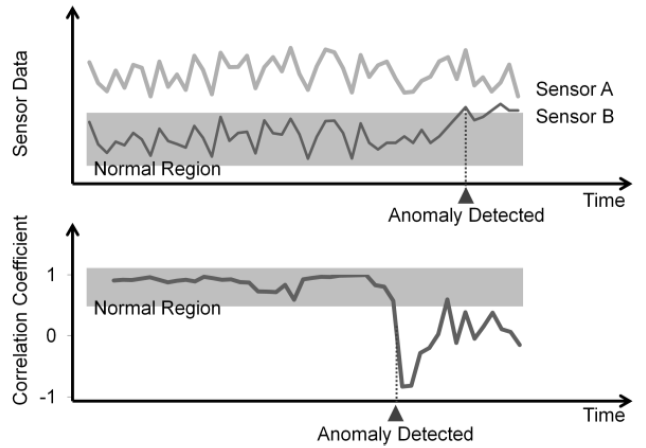
\includegraphics[width=0.65\textwidth]{Figures/Chapter03/Fig.03.34_Correlation.png}
	\caption{Anomaly detection using correlation coefficient \parencite{zhao2017advanced}}
	\label{fig03.34}
\end{figure}

In general, an anomaly in a system is any abnormal behavior of the system. According to Lopez et al., \textit{an anomaly is an occurrence that is different from what is standard, normal, or expected} \parencite{lopez2017categorization}. As shown in Fig. \ref{fig03.35}, the root cause of anomalies is not only machine failures. The reason can also be broken sensors, errors of SCADA system/network, cyber-attacks and so on.

According to Lopez et al., Semi-supervised anomaly detection are Semi-supervised methods use normal data sets to train models of normal behavior, and label any observations that deviate significantly from those models as anomalies \parencite{lopez2017categorization}.

In a data-driven anomaly detection system, a high occurrence of anomalous data can be considered as anomalies. For Predictive Maintenance problem, anomalies can be early signs of machine failures.

\begin{figure}[h]
	\centering
	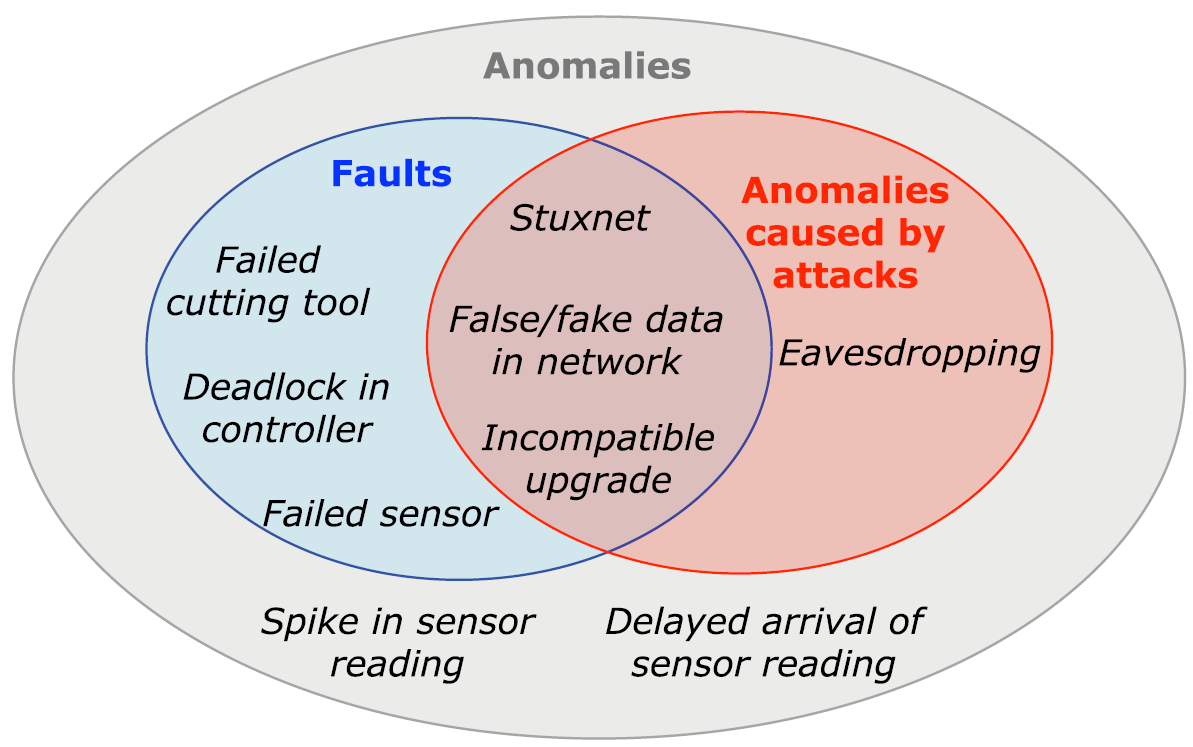
\includegraphics[width=0.65\textwidth]{Figures/Chapter03/Fig.03.35_Anomaly.png}
	\caption{Anomalies in Smart Manufacturing \parencite{lopez2017categorization}}
	\label{fig03.35}
\end{figure}

In principle of semi-supervised Anomaly Detection methods, the model will be trained with data of normal conditions in a certain way so that it can detect if new data is anomalous. In some researches, Anomaly Detection model is also called Normal Behavior Model (NBM) because it learns machines or systems in normal conditions \parencite{roelofs2021autoencoder} \parencite{serradilla2021adaptable}. 

Fig. \ref{fig03.36} is a general learning and prediction process of a Normal Behavior Model (NBM) presented by Pollak et al. \parencite{pollak2021prediction}.

\begin{figure}[h]
	\centering
	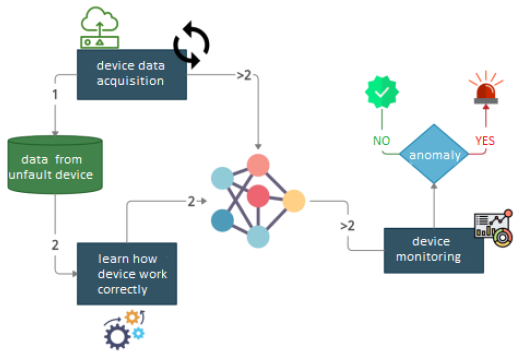
\includegraphics[width=0.85\textwidth]{Figures/Chapter03/Fig.03.36_NBM.png}
	\caption{Normal Behavior Model for Anomaly Detection \parencite{pollak2021prediction}}
	\label{fig03.36}
\end{figure}

Critical condition of this approach is that the normal behavior model must be trained by normal data. Normal data is data of un-fault device (or data of normal working conditions) \parencite{pollak2021prediction} \parencite{tedesco2021scalable}. If there are anomalous data mixed in training data, the model will receive undesired training and not be able to recognize anomalies effectively in the future.

Machine data is acquired by Wireless Sensor Network (WSN) and SCADA system. WSN and SCADA are parts of the industrial system. They can also have failures and can generate anomalous data. There are studies about anomaly detection for SCADA system \parencite{nazir2021autoencoder} and WSN \parencite{luo2018distributed}. However, it is not in the scope of this work. Most of studies of anomaly detection for industrial machines rely on the condition that WSN and SCADA work well. In case there are anomalous data generated by other reason, anomaly notification raised by the model is simply skipped because they are false alarms. If these anomalous data were used for training the model, they must be excluded from training data and the model must be re-trained.

How to select normal data for training and re-training the models will be presented in details in Chapter \ref{Chapter5}. It is an important aspect of using predictive models in real life.

Various techniques of different theories can be used to model the anomaly detection problem. For example, Zhao et al. use statistical model to discover statistical distributions of correlations of sensor data \parencite{zhao2017advanced}. Among Machine Learning algorithms, the current best-in-class Outlier Detection algorithm is Isolation Forest \parencite{alfeo2020using}. 

Two popular learning-based methods are Regression model and AutoEncoder. In Regression method, the models try to predict an output or a dependent variable using related input variables, while AutoEncoder-based models try to reconstruct input data. Regression models can be implemented by either Machine Learning algorithms or Deep Learning models, while AutoEncoder is Deep Learning model. Although Regression method is not chosen in this work, it is briefly presented here for comparison.


\subsection{Regression models for Anomaly Detection} \label{part3.3.4}

Moleda et al. build an anomaly detection system for early detection of faults in Boiler Feed Water Pumps in power plant \parencite{moleda2020predictive}. These pumps are parts of continuous manufacturing process of electricity production (Fig. \ref{fig03.37}).

\begin{figure}[h]
	\centering
	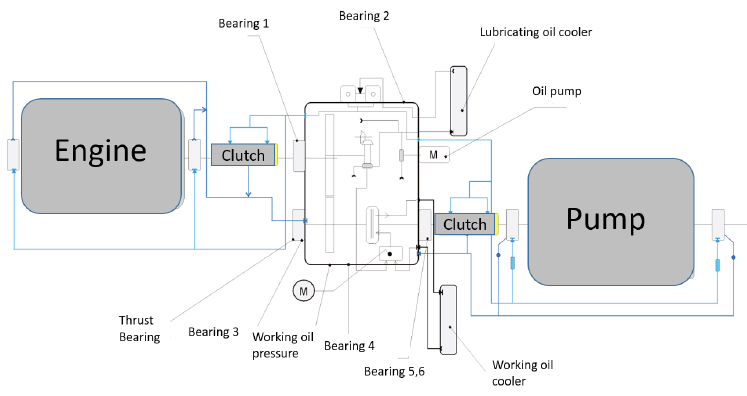
\includegraphics[width=0.9\textwidth]{Figures/Chapter03/Fig.03.37_Regression.png}
	\caption{Boiler Feed Water Pumps in power plant \parencite{moleda2020predictive}}
	\label{fig03.37}
\end{figure}

Moleda et al. implement their regression model using their own algorithms. Input are 22 variables, mostly temperature and pressure, while output is value of the water flow behind the pump. The regression model is trained with historical data of good conditions acquired by SCADA system. 

In order to predict anomalies, predicted values by the regression model are compared to real values. If the gap between predicted values and real values of water flow has the trend to increase, it can be an early sign of failures.

\begin{figure}[htp]
	\centering
	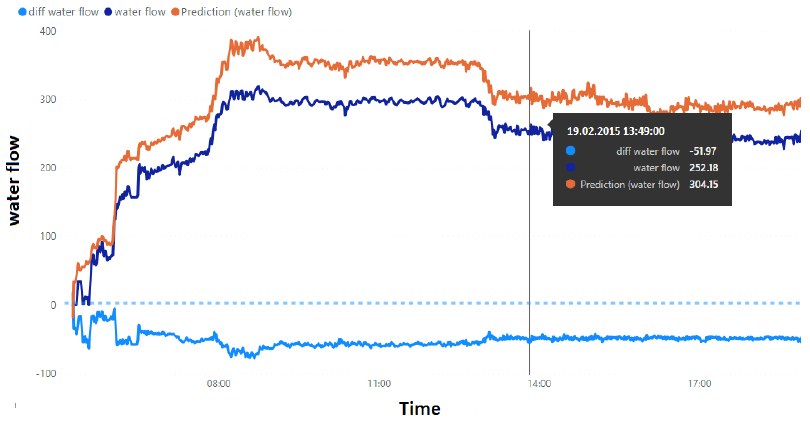
\includegraphics[width=\textwidth]{Figures/Chapter03/Fig.03.38_Regression.png}
	\caption{Real and estimated value of the water flow behind the pump \parencite{moleda2020predictive}}
	\label{fig03.38}
\end{figure}

Another example of regression method is regression model for detect anomalies for photovoltaic panels of solar power plant by Huuhtanen et al. \parencite{huuhtanen2018predictive}. In this case, output is amount of electric power a panel should generate while input is historical data of that panel, local weather information and electricity power generated by neighboring panels. The regression model is implemented by Convolutional Neural Network (CNN). However, regardless which technique is used, the idea is similar.

Regression method, in case it can be developed, will be very efficient. It usually uses selective input variables for training the regression model, leading to computational simplicity. Regression model can be implemented by both Machine Learning or Deep Learning. Especially, its result is very human readable, without sophisticated interpretation. 

However, in regression method, an explicit output, or a dependent variable, needs to be known. This condition can difficult, or it's even impossible, in many cases (e.g. belt drive in study by Pollak et al. \parencite{pollak2021prediction}).

Moreover, in order to select input and output variables and verify their dependency, a certain level of knowledge of the machine is needed (Fig. \ref{fig03.37}, for example). This is a little like the hybrid approach between physical model-based approach and data-driven approach.

For building a data-driven anomaly detection solution with minimal requirement of machine knowledge, the AutoEncoder-based method is more suitable. The approach using AutoEncoder is more general and scalable. As a trade-off, it will be heavier because AutoEncoder is a complex Deep Learning architecture.

For these reasons, AutoEncoder-based method is chosen for the Anomaly Detection solution in this work.


\section{AutoEncoder for Anomaly Detection} \label{part3.4}

\subsection{Anomaly Detection based on Data Reconstruction Error}

As illustrated in Fig. (Fig. \ref{fig03.39}), in semi-supervised anomaly detection approach, after models are trained with machine data of normal operating conditions, machine health indicators of normal data will be calculated and then a threshold will be set. With new data, these indicators will be calculated. If values of these indicators of new data are above the threshold, new machine data are considered as anomalous data and can be signs of coming failures.

\begin{figure}[h]
	\centering
	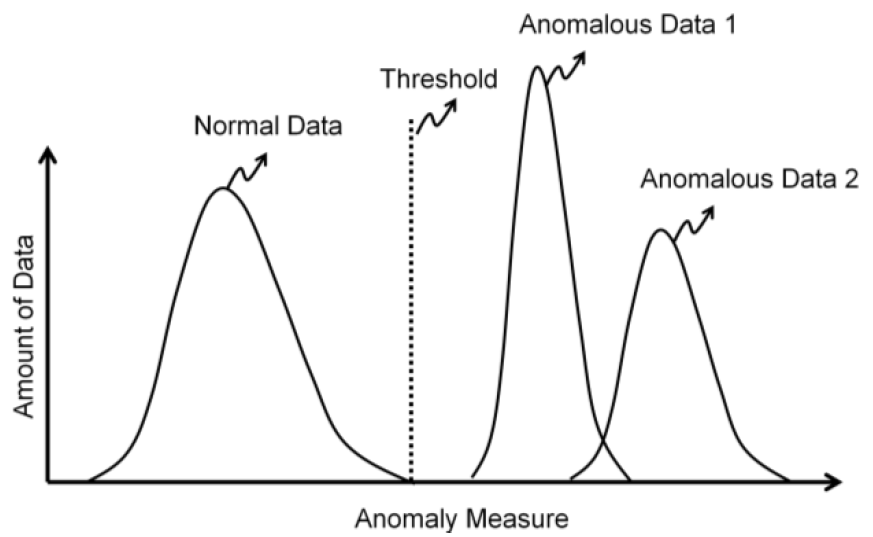
\includegraphics[width=0.65\textwidth]{Figures/Chapter03/Fig.03.39_Anomaly_Detection.png}
	\caption{Anomaly Detection \parencite{zhao2017advanced}}
	\label{fig03.39}
\end{figure}

Percentage of anomalous data (having health indicators above the threshold) is called Anomaly Measure (or Anomaly Score). Depending on the chosen technique, the anomaly score is monitored and if it is higher than the threshold of normal condition during a continuous monitoring time range, the current condition of the machine can be anomaly.

In the Deep Learning approach using AutoEncoder, the anomaly score is calculated from data Reconstruction Error (Fig. \ref{fig03.40}).

\begin{figure}[h!]
	\centering
	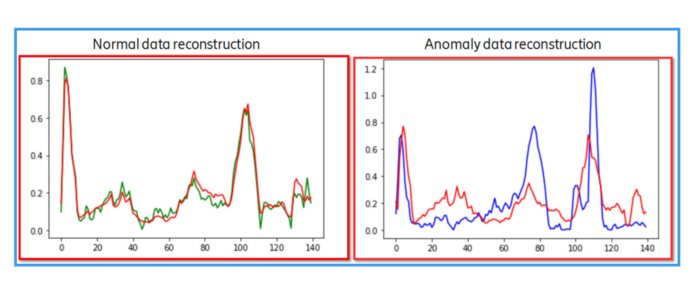
\includegraphics[width=\textwidth]{Figures/Chapter03/Fig.03.40_RE.png}
	\caption{Anomaly Detection based on Data Reconstruction Error (\url{https://medium.com/@Sanath_raj/anomaly-detection-using-autoencoders-ad92aa0493d3})}
	\label{fig03.40}
\end{figure}

\subsection{Introduction of AutoEncoder}

AutoEncoder (AE) are Neural Network type that can reconstruct the input. An Autoencoder is a feed forward neural network in which the desired output is the input itself. AE is able to tackle unsupervised tasks, and for this reason are strongly used for anomaly detection \parencite{tedesco2021scalable}. Fig. \ref{fig03.41} is the basic schematic diagram of the AutoEncoder. 

\begin{figure}[h]
	\centering
	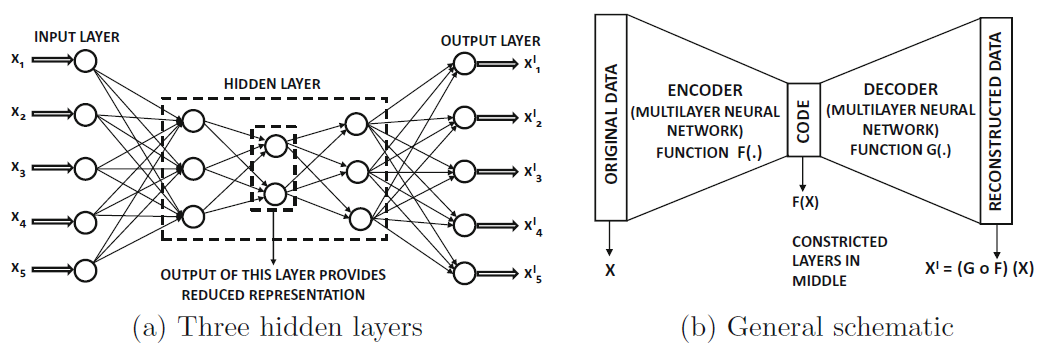
\includegraphics[width=\textwidth]{Figures/Chapter03/Fig.03.41_AE.png}
	\caption{The basic schematic of the autoencoder \parencite{aggarwal2018neural}}
	\label{fig03.41}
\end{figure}

The typical AE structure is subdivided into three main parts \parencite{tedesco2021scalable}:

- Encoder: neural network that has the goal to learn how to encode the original data in a low dimensional representation;

- Bottleneck Layer: the layer that contains the coded reduced representation. Content of this layer is the latent representation of input data.

- Decoder: neural network that has the goal to reconstruct from the bottleneck representation the original data in the most possible way.

\begin{figure}[h]
	\centering
	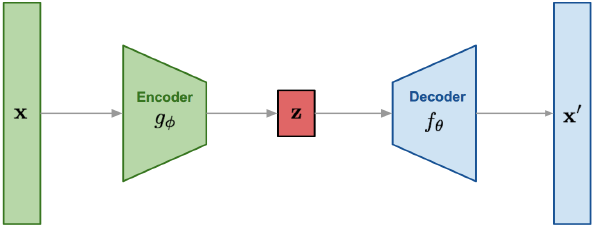
\includegraphics[width=0.85\textwidth]{Figures/Chapter03/Fig.03.42_AE.png}
	\caption{Structure of AutoEncoder \parencite{pollak2021prediction}}
	\label{fig03.42}
\end{figure}

Fig. 3.42 is the mathematic presentation of the AutoEncoder, of which:

- x is original input data.

- z is the \textbf{latent representation} (reduced dimensional data) of the original data: z = g(x). z is also called \textbf{latent vector}.

- x’ is the reconstructed data from reduced dimensional data: x’ = f(z)

The full data transformation of the AutoEncoder will be: y = f(z) = f(g(x))

Because in AutoEncoder, expected output is also input, the objective of the training process will be:
\[ x’ = x \Leftrightarrow f(g(x)) = x \]

The distance between original input data x and reconstructed data x’ is Reconstruction Error (RE). RE is measured by loss function L(x, x’). L can be simple distance formula such as Mean Absolute Error (MAE), Mean Squared Error (MSE), Root Mean Squared Error (RMSE) or more complicated distance formula such as Mahalanobis distance  \parencite{lutz2020evaluation}. The most popular distance used is MSE:
\[
L(X,X^{'}) = \frac{1}{n}\sum_{i=1}^{n}(x_{i}-x^{'}_{i})^{2}
\]
% S(z)_{i} = \frac { e^{z_{i}} } { \sum_{j=1}^{k} e^{z_{j} } }

Training the AutoEncoder is the progress of minimizing the lost function L(X, X’).

In order to achieve this objective, the structure of an AutoEncoder must comply these constraints:

- Input and output layers (first and last layers) must have the same size

- The size of the latent representation layer must be much smaller than the size of the input and output layers (otherwise, it is just the copy of the input)

- The number of nodes in each layer decreases from the input layer to the representation layer and then increases from the representation layer to the output layer 

Besides these constraints, the implementation of AutoEncoder is quite free. Therefore, AutoEncoder is actually a Deep Learning architecture more than a concrete Deep Learning type because it can be implemented by any of three popular Deep Learning types: Feed Forward Neural Network (MLP), Convolutional Neural Network (CNN) or LSTM.

There are variations of AutoEncoder. The standard form is UnderComplete AutoEncoder (UC AE). It can be implemented by a basic FFNN ((Fig. \ref{fig03.43})).

\begin{figure}[h]
	\centering
	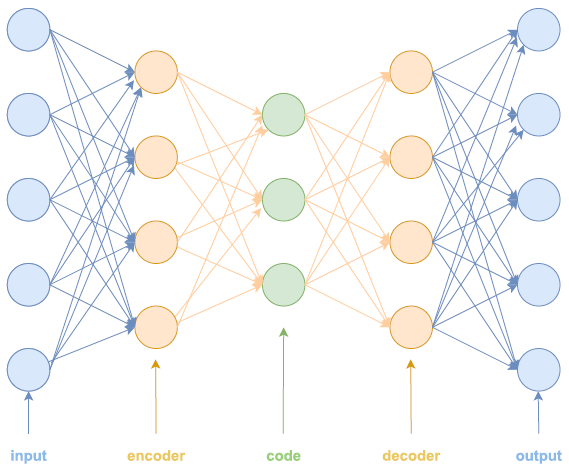
\includegraphics[width=0.8\textwidth]{Figures/Chapter03/Fig.03.43_AE.png}
	\caption{Basic architecture of an AE \parencite{jebril2022autoencoder}}
	\label{fig03.43}
\end{figure}

One popular variation of AutoEncoder is Variational Autoencoder (VAE). In VEA, the Mean and Standard Deviation vectors are inserted as a layer before the latent vector. With this modification, VAE become a Generative Adversarial Network (GAN) because it can generate new content that looks alike original content.

AutoEncoder has different applications, besides anomaly detection and content generation. An example is data denoising. In data denoising application, UnderComplete AutoEncoder is used but original data is corrupted (noise added) before being used as input for training. The expected output is still original data. The objective of the training process become
\[ f(g(x_{corrrupted}) = x \]
so that the trained AE will be able to convert corrupted data to clean data.

\begin{figure}[h]
	\centering
	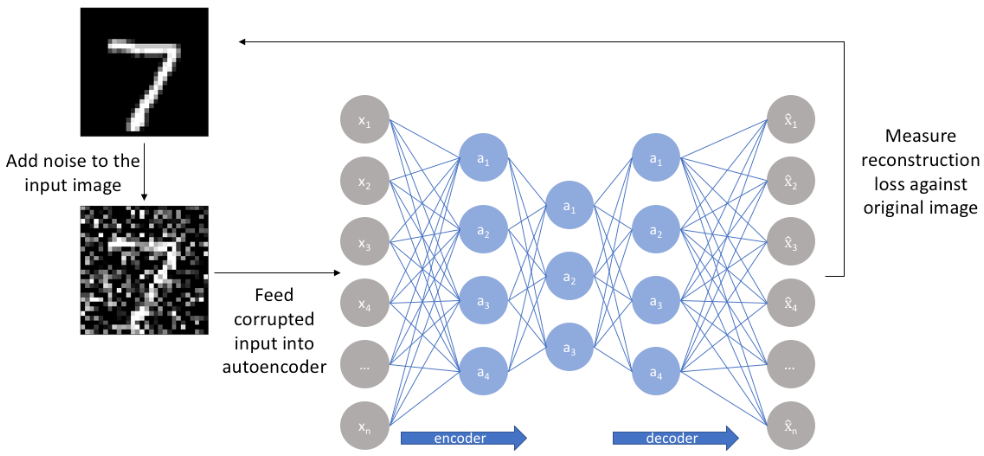
\includegraphics[width=\textwidth]{Figures/Chapter03/Fig.03.44_Denoise.png}
	\caption{Denoising AutoEncoder (\url{https://www.jeremyjordan.me/autoencoders/)}}
	\label{fig03.44}
\end{figure}

One of most advanced application of AutoEncoder architecture is the Spatio-temporal AutoEncoder for video anomaly detection proposed by Zhao et al. \parencite{zhao2017spatio}.

\begin{figure}[h]
	\centering
	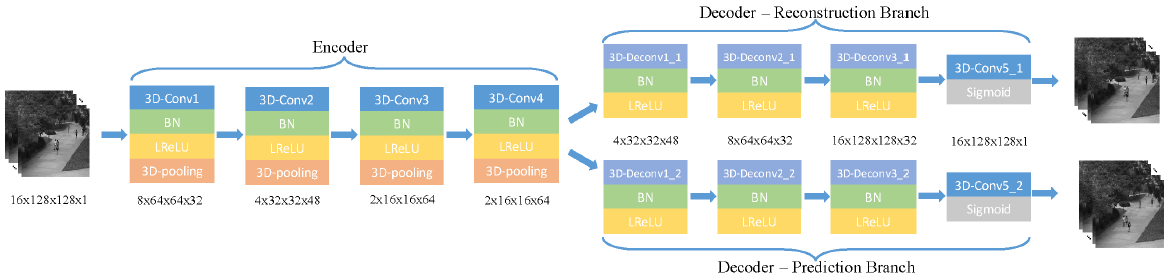
\includegraphics[width=\textwidth]{Figures/Chapter03/Fig.03.46_AE_Spatio.png}
	\caption{Spatio-temporal AutoEncoder for video anomaly detection \parencite{zhao2017spatio}]
	}
	\label{fig03.46}
\end{figure}

AutoEncoder can be used in replacement of dimensional reduction algorithms because they share the same principle: reduce dimensions of data with minimum information loss. Instead of original x, latent representation z can be used as input for other applications such as classification (Fig. \ref{fig03.45}).

\begin{figure}[h!]
	\centering
	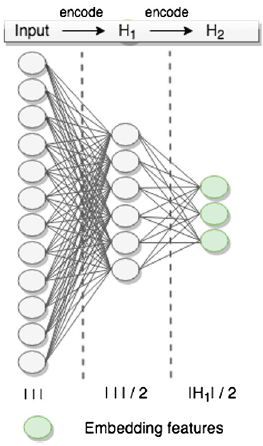
\includegraphics[width=0.35\textwidth]{Figures/Chapter03/Fig.03.45_Reduce.png}
	\caption{Feature extraction using the encoding function of AE \parencite{corizzo2019anomaly}}
	\label{fig03.45}
\end{figure}

The terminology AutoEncoder (AE) or Deep AutoEncoder (DAE) often refers to the Under-Complete AutoEncoder. For Anomaly Detection, only UnderComplete AutoEncoder is needed because it tries to reconstruct exactly the input.

UnderComplete AutoEncoder can be implemented using standard FFNN or more complicated Deep Learning models such as CNN and LSTM.

LSTM is powerful for predictive models of time-dependent sequential data. If machine data has time dependency (e.g. machine running in cycles like 4-stroke engine or continuous production lines), LSTM can be used for implementation of AutoEncoder.

Dallapiccola implements an AutoEncoder using LSTM for time-dependent data \parencite{dallapiccola2020predictive}. This model is designed for predictive maintenance of centrifugal pumps. Failure is predictive by Reconstruction Error of $n$ multivariate data samples collected by 80 sensors put on the monitor pumps (Fig. \ref{fig03.47}).

\begin{figure}[h!]
	\centering
	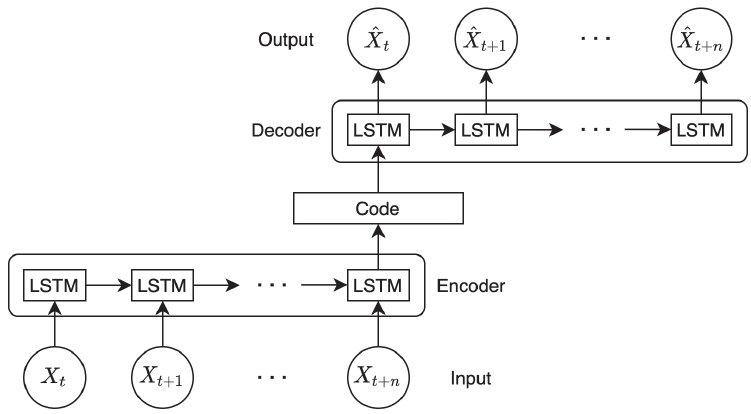
\includegraphics[width=0.8\textwidth]{Figures/Chapter03/Fig.03.47_LSTM.png}
	\caption{LSTM AutoEncoder for Centrifugal Pumps predictive maintenance \parencite{dallapiccola2020predictive}]
	}
	\label{fig03.47}
\end{figure}

In case time dependence is not clear and the FFNN is not powerful enough, CNN can be used.
CNN is a variation of Feed Forward Neural Network specialized for image classification. The idea is to split the image to smaller part for recognition. For example: a human face must have two eyes above nose and mouth. Fig. \ref{fig03.49} is the vehicle image classification implemented by CNN.

\begin{figure}[h]
	\centering
	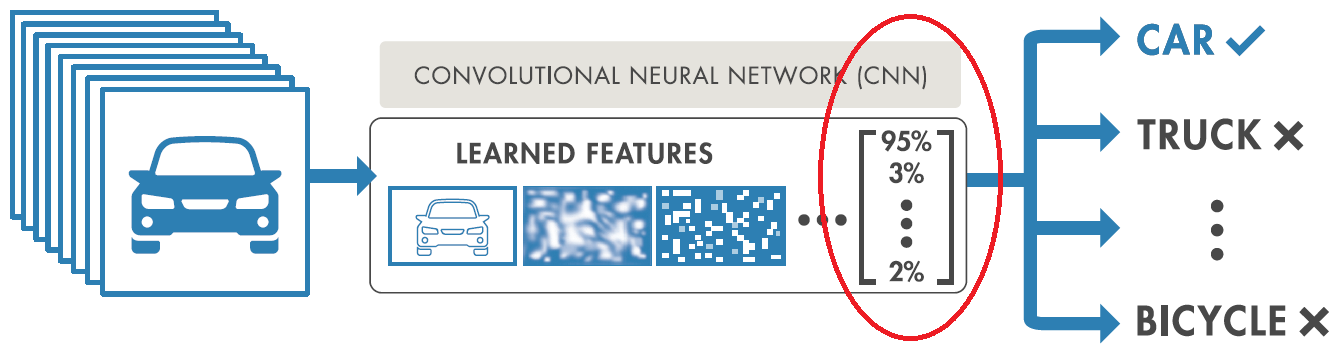
\includegraphics[width=0.7\textwidth]{Figures/Chapter03/Fig.03.49_Classification.png}
	\caption{An image classifier implemented by CNN (source: MathWorks)}
	\label{fig03.49}
\end{figure}

Yuan et al. implement an AutoEncoder using 2D CNN for predictive maintenance also by monitoring Reconstruction Error \parencite{yuan2017deep}. 2D input data is multi-feature sequence data. The first dimension is the list of sensor and the second dimension is time dimension.

\begin{figure}[h!]
	\centering
	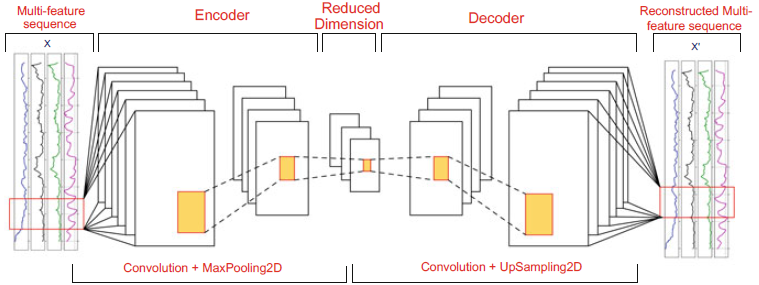
\includegraphics[width=\textwidth]{Figures/Chapter03/Fig.03.48_3D.png}
	\caption{Anomaly Detection AutoEncoder implemented by 2D CNN \parencite{yuan2017deep}]
	}
	\label{fig03.48}
\end{figure}

\begin{figure}[h!]
	\centering
	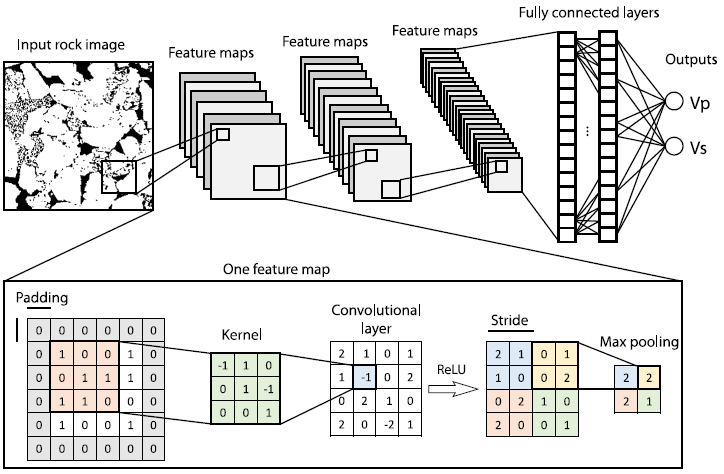
\includegraphics[width=0.8\textwidth]{Figures/Chapter03/Fig.03.50_CNN.png}
	\caption{Schematic illustration of a convolutional neural network \parencite{karimpouli2019image}}
	\label{fig03.50}
\end{figure}

Fig. \ref{fig03.50} is an illustration of the way a CNN extracts image hidden feature for classification. CNNs are based on a large number of convolutional layers (i.e., features maps) obtained from convolution of image by many small size kernels. These huge numbers of kernels extract a vast number of features that are hidden in the image \parencite{karimpouli2019image}.

The ability to extract hidden features of CNN can be utilized for implementation of AutoEncoder. Combining them to the AutoEncoder architecture, we have the structure as Fig. \ref{fig03.51}. Each layer of the AutoEncoder is a pair of a Convolutional layer and a Pooling layer. This Deep Learning architecture is called Convolutional Deep AutoEncoder (CDAE).

\begin{figure}[h!]
	\centering
	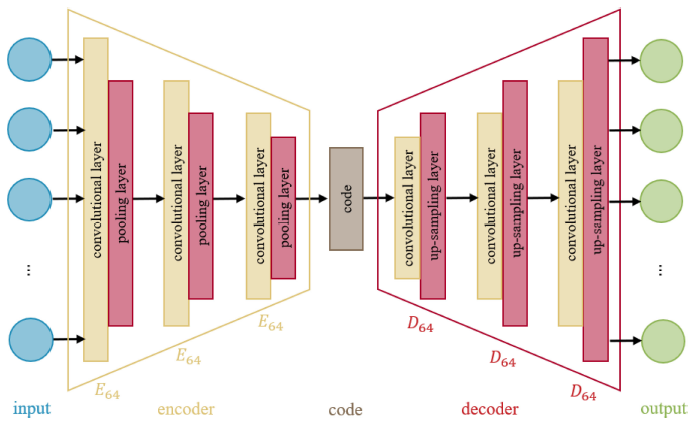
\includegraphics[width=\textwidth]{Figures/Chapter03/Fig.03.51_CDAE.png}
	\caption{Convolutional Deep AutoEncoder \parencite{jebril2022autoencoder}}
	\label{fig03.51}
\end{figure}

Convolutional Deep AutoEncoder (CDAE) is chosen for implementation of the proposed solution of this work. In the rest of this chapter, more details of the way how AutoEncoder can be used for anomaly detection is presented, together with introduction of some studies using this method.


\subsection{AutoEncoder-based Anomaly Detection method} \label{part3.4.3}

The AutoEncoder-based anomaly detection method relies on the fact that AutoEncoder has a very high ability in remembering and comparing patterns. After the training process, the trained AutoEncoder will be used to create reconstruction error of new data in order to calculate the anomaly score. Data with high reconstruction error score are considered as anomalous data because only normal data are used to train the AutoEncoder. The AutoEncoder, by correctly fitting undamaged data, can reconstruct normal data very well, while it can not do so with anomalous data that it has not encountered \parencite{pollak2021prediction}. The ability to reconstruct training data of the AutoEncoder is illustrated in Fig. \ref{fig03.52}.

\begin{figure}[h]
	\centering
	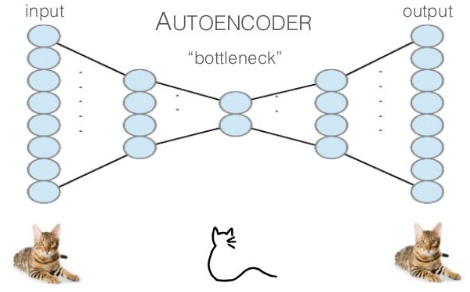
\includegraphics[width=0.6\textwidth]{Figures/Chapter03/Fig.03.52_Cat.png}
	\caption{Latent representations in an autoencoder (\url{http://www.cs.us.es/~fsancho/?e=232)}}
	\label{fig03.52}
\end{figure}

Fig. \ref{fig03.53} the general flow of anomaly detection approach using AutoEncoder.

\begin{figure}[h]
	\centering
	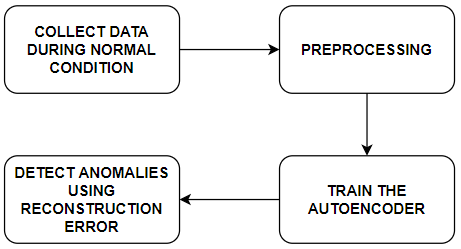
\includegraphics[width=0.6\textwidth]{Figures/Chapter03/Fig.03.53_AD.png}
	\caption{AutoEncoder-based anomaly detection approach \parencite{tedesco2021scalable}}
	\label{fig03.53}
\end{figure}

\textbf{Step 1 - Collect data during normal condition}: First, a training dataset of normal operating condition of machines need to be prepared. The most important thing of this step is to make sure that only data of normal conditions are collected. Data of testing, maintenance, set up, special time (e.g. there is a storm), wireless sensor network or SCADA error must be excluded.

\textbf{Step 2 - Preprocessing}: Second step is data preprocessing. For an effective anomaly detection solution, the AutoEncoder training dataset must be as cleaned as possible. It should be cleansed from noise and especially anomalies through an extensive preprocessing step. If this preprocessing step is not effective, the AutoEncoder will learns also anomalous data, and obviously in future it will recognize anomalous data as normal data.

Preprocessing step includes but not limited these tasks: remove constant and noisy signals, drop signals with high empty data gap, change all signal to the same frequency, data imputation (deal with empty value), data scaling and so on.

Tedesco21 et al. also suggest to remove high correlated columns \parencite{tedesco2021scalable}. However, we are not really convinced with that idea. The reason and anti-example will be presented in Chapter \ref{Chapter3}.

\textbf{Step 3 - Train the AutoEncoder}: Once data are already preprocessed, these data will be used for training the AutoEncoder. The input and output size of AutoEncoder depends on how many signals are kept for anomaly detection.

In principle, a model is used dedicatedly for only one machine, although the machine can be a complex machine (for example: the real case study of Wind Turbine presented in Chapter \ref{Chapter7}). 
Exceptions can be simple devices such as light or fan. However, in general it should be avoided. Two machines of the same type, same configuration, at the same industrial site... does not means that data of this machine can be used to predict failures of the other, nor their data can be mixed. Machines of same type can have the same training dataset structure and same AutoEncoder structure for simplicity, but not the same trained model.

\textbf{Step 4 - Detect Anomalies using Reconstruction Error}: Once the AutoEncoder is trained, it can be used for anomaly detection by comparing Reconstruction Error of new operating data with Reconstruction Data of training data. Following is exactly what have to be done.

First, we have the training dataset $X_{normal}$ of the machine. It will be used to train the AutoEncoder. Once the training process is converged, we have the trained AutoEncoder.

Then the trained AutoEncoder will be used to reconstruct the training dataset $X_{normal}$. The output will be $X_{normal}^{'}$.

Then the Reconstruction Error (RE) of training dataset, call $RE_{normal}$, will be calculated, using the loss function L (e.g. MSE):
\[ RE_{normal} = L(X_{normal}, X_{normal}^{'}) \]
We use the $RE_{normal}$ as the baseline for comparison with Reconstruction Error of new data.

Until this step, we have 2 results: the trained AutoEncoder and the Reconstruction Error set of normal data. These two results can be deployed for anomaly detection.

New data of the monitored machine during a time range (e.g. hours, days, weeks, months…), called $X_{new}$, will be preprocessed in the same way as the training dataset. Then the AutoEncoder will be used to reconstruct this dataset. The output will be $X_{new}^{'}$. Then the Reconstruction Error of the new dataset will be calculated with the same way:
\[ RE_{new} = L(X_{new}, X_{new}^{'}) \]
At this step, we have on hand two Reconstruction Error sets of normal data and new data. The mission is to compare them in a certain way (mostly by a statistical/mathematical methods) in order to decide if there are anomalies in new machine data. 

There are many advanced analytics techniques for analyzing the result. However, one simple ways is to display the two Reconstruction Error sets in histogram (Fig. \ref{fig03.54}).

\begin{figure}[h]
	\centering
	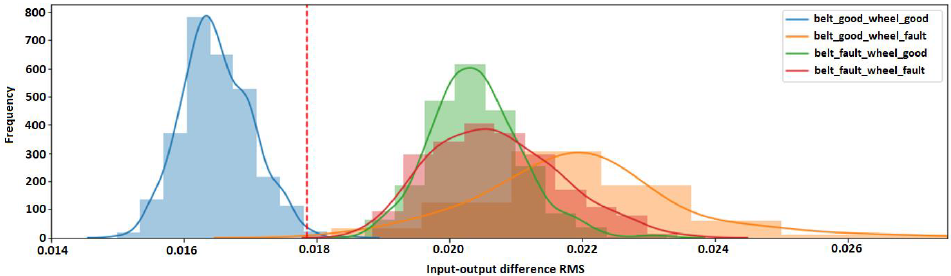
\includegraphics[width=\textwidth]{Figures/Chapter03/Fig.03.54_Histogram.png}
	\caption{Distribution of reconstruction error for each damage-related class for vertically positioned sensor \parencite{pollak2021prediction}}
	\label{fig03.54}
\end{figure}

Fig. \ref{fig03.54} is the result of the study by Pollak21 et al., also using AutoEncoder-based method for detecting anomalies of belt drive \parencite{pollak2021prediction}. The vertical dotted line is the Reconstruction Error threshold (RE Threshold) so that only a small percentage of training data has Reconstruction Error (RE) higher than this threshold. This targeted percentage is usually small, about 3\%-7\%, and can be called Anomaly Threshold. If RE of a new data sample is higher than the RE Threshold, it will be considered as anomalous data. \% anomalous data of new data during a continuous time range will be monitored and compared to the Anomaly Threshold.

Because Fig. \ref{fig03.54} are simulated failures, most of new data samples exceed the RE threshold. In real cases, if about 10\%-15\% of new data has RE above the RE threshold, an alarm can be raised. 

In summary, there are two thresholds. The Reconstruction Error threshold is used to determine if a data sample is anomalous (if its RE is higher than this RE threshold). The Anomaly Threshold defines how much anomalous data in a continuous monitoring time range can be considered as anomaly.

If these thresholds are set too strict, the AutoEncoder can generate too many false alarms. However, if they are too easy, we may not be able to predict some failures. The choice depends on the opinions of stakeholders and how critical the machine is. For example, for SCADA system, false alarms are preferred than undetected anomalies \parencite{nazir2021autoencoder}. In the case study presented in Chapter \ref{Chapter7}, wind turbines are on the sea, so verifying a false alarm can be easier than coming to the wind power plant to fix a failure.

Compared to the regression method, the Anomaly Detection method using AutoEncoder is much easier to deploy. It is useful to have machine expertise but it's not mandatory. We only need to collect signals related to machine status for learning. These data can be read through I/O module of the machine or we can install sensors around the machine in order to collect machine condition indicators such as vibration, temperature, pressure, noise… For example, in the study by Pollak et al., they simply put vibration sensors on the surface of the belt drive \parencite{pollak2021prediction}. 

\begin{figure}[h!]
	\centering
	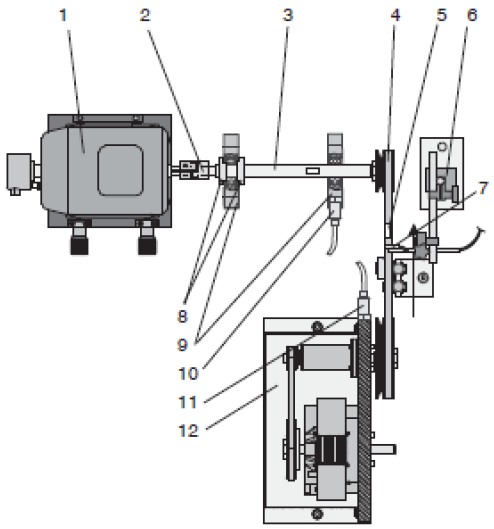
\includegraphics[width=0.55\textwidth]{Figures/Chapter03/Fig.03.55_belt.png}
	\caption{Setup for simulation of vibrations from belt drive \parencite{pollak2021prediction}}
	\label{fig03.55}
\end{figure}

They conduct two experiments: one with sensors installed vertically and one with sensors installed horizontally. Fig. \ref{fig03.54} is the result of vertically positioned sensor experiment while Fig. \ref{fig03.56} is result of horizontally positioned sensor experiment. Both manners of sensor installation show positive results. In this study, only vibration sensors are used. If there are sensors of different types, the ability to detect anomalies will be much more powerful.

\begin{figure}[h]
	\centering
	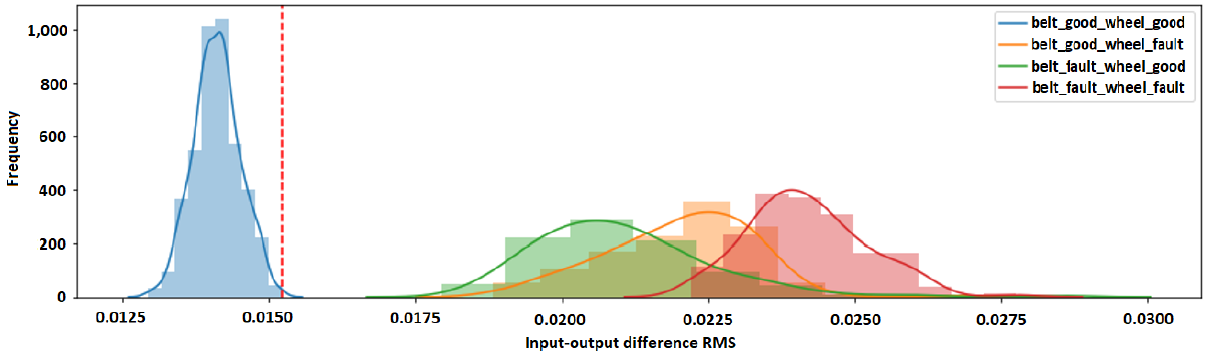
\includegraphics[width=\textwidth]{Figures/Chapter03/Fig.03.56_histogram.png}
	\caption{Distribution of reconstruction error for each damage-related class for horizontally positioned sensor \parencite{pollak2021prediction}}
	\label{fig03.56}
\end{figure}

Easy to deploy is the advantage of the Anomaly Detection method using AutoEncoder. However, it has its own challenges. If these challenges are not resolved, the solution cannot be used efficiently in real life.

The first difficulty is to set the anomaly threshold. We need to balance between false alarm and undetected failures, especially if the solution is deployed for a big number of machines. Alfeo et al. try to automate the determination of this threshold so that the anomaly detection solution will have better adaptation capability \parencite{alfeo2020using}.

The second challenge is the false alarm caused by the phenomenon of Model Drift (or Model Degradation). It is the scenario that the model trained by obsolete data cannot process new data correctly \parencite{bayram2022concept}.

AutoEncoder-base anomaly detection method is based on data Reconstruction Error concept. If the AutoEncoder cannot reconstruct new data, it only means that the new data is not similar to any pattern of the training data. It is not possible to conclude that the new data is generated by a potential failure. Maybe, the new data is simply data of new normal operating conditions. In this case, false alarms are generated by the Model drift (Fig. \ref{fig03.57}).

\begin{figure}[h!]
	\centering
	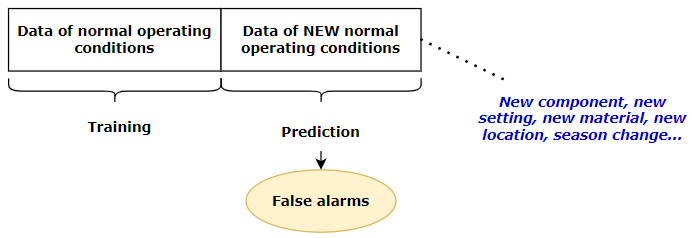
\includegraphics[width=0.9\textwidth]{Figures/Chapter03/Fig.03.57_Drift.png}
	\caption{False alarms generated by Model Drift}
	\label{fig03.57}
\end{figure}

In other applications such as image classification, in order to avoid model drift, we can simply re-train the model with newer data, the more frequent training the better. However, in the AutoEncoder-base anomaly detection solution, re-training the AutoEncoder with too "new" data have the risk that the AutoEncoder can learn data of potential failures. Studies show that before a failure happens, its root cause could start months ago and anomalous data was increasing gradually \parencite{bengtsson2018importance}.

\begin{figure}[h!]
	\centering
	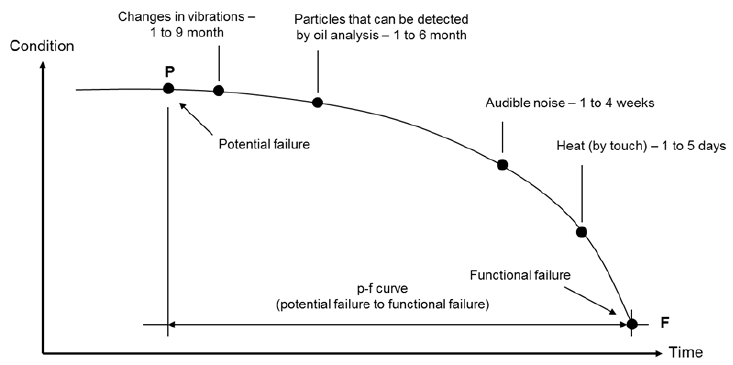
\includegraphics[width=\textwidth]{Figures/Chapter03/Fig.03.58_Curve.png}
	\caption{Example of a p-f curve of a ball bearing \parencite{bengtsson2018importance}}
	\label{fig03.58}
\end{figure}

When the root cause (or the degradation) started, anomalous data was not enough for being detected. If the AutoEncoder was re-trained with that anomalous data, the AutoEncoder will never be able to detect this failure or the failure will be detected too late for avoiding (Fig. \ref{fig03.59}).

\begin{figure}[h!]
	\centering
	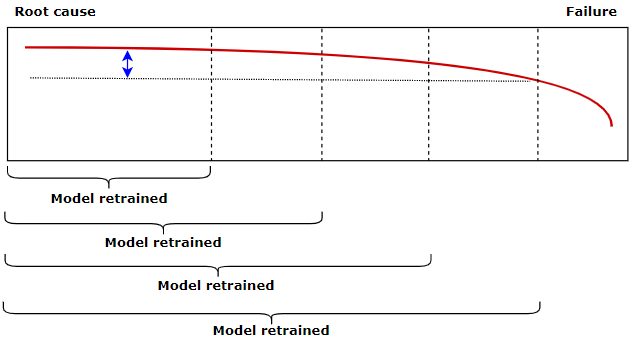
\includegraphics[width=0.9\textwidth]{Figures/Chapter03/Fig.03.59_risk.png}
	\caption{Risk of AutoEncoder being trained by failure data}
	\label{fig03.59}
\end{figure}

These difficulties are rarely met when testing the solution with experimental dataset or simulated failures, but when deploying the anomaly detection solution for real cases, the dilemma between risk of false alarm and risk of undetected failures needs a strategy to balance. The decision needs the involvement of real users of the Predictive Maintenance solution. Although at the first look, false alarms seem to be less serious, in long term users can ignore alarms raised by the solution and finally not use the solution anymore.

Despite these challenges, AutoEncoder-based Anomaly Detection method is a very successful technique for the Predictive Maintenance problem. Many studies justify its capability of detecting anomalies of complex industrial machines.

AutoEncoder-base Anomaly Detection method is not an unsupervised learning method, like clustering models which can work with all collected data. It is the semi-supervised learning method because it needs training data of only good working conditions, like for a binary classification mode. However, compared to supervised learning that need labeled and balanced data, training data requirement for AutoEncoder-based Anomaly Detection method is much easier. Therefore, this approach has high feasibility for deployment in real life. Many studies of Anomaly Detection using this approach can be tested with real case studies \parencite{roelofs2021autoencoder} \parencite{alfeo2020using} \parencite{serradilla2021adaptable} \parencite{lutz2020evaluation} \parencite{tedesco2021scalable}.

\subsection{Referenced studies of Anomaly Detection using AutoEncoder}

\textbf{A scalable deep learning-based approach for anomaly detection in semiconductor manufacturing} \parencite{tedesco2021scalable}

Tedesco et al. propose a general and scalable AutoEncoder-based approach for anomaly detection in semiconductor manufacturing, a very complex manufacturing industry. Primary steps of their approach are already presented in \ref{part3.4.3} (Fig. \ref{fig03.53}).
%As already described, the key idea behind the AE-based anomaly detection method is to measure how far the data reconstructed by the trained AE are from the input data.

The main strength of this approach is its generality and scalability because it is not based on specific characteristics of any dataset, machines or industrial process. Therefore, it can be used to handle heterogeneous datasets come from different equipment, work centers and even production sites. They consider the Anomaly Detection problem as multivariate problem without time dependency. They not only propose an approach but also describe details of their implementation with recommended best practices.

First, in data processing step, they propose to remove constant (or N/A) columns, highly correlated columns and nosy columns of the training dataset. Noise features can be removed by the Kolmogorov-Smirnov (KS) test presented Andrey Kolmogorov and Nikolai Smirnov in 1933. Then the training dataset must be scaled. This step is also called Data Normalization so that all features belong to the same value range, otherwise the calculation of the distance will not be correct.

They also shuffle randomly the training dataset in order to remove any possible time dependence in the data. The motivation of this step is that except data is clearly known as time-dependent and a time dependent approach is chosen, they don't want the AutoEncoder to learn any time dependencies. Each training data sample (or a continuous block of data sample called data window) will be learnt by Deep Learning model as a separate snapshot of the machine condition.

They also recommend an initial hyperparameter set which can start with most of AutoEncoder models. First, the percentage used in splitting process is 90\% (90\% for the training set and 10\% for the test set). The default loss function used for training and evaluation can be Mean Squared Error (MSE). The optimizer can be Adam optimizer (Adaptive Moment Estimation, an improvement of Stochastic Gradient Descent (SGD) algorithm). Early Stopping strategy can be used to perform regularization and avoid overfitting. Although ReLU activation function is often used for AutoEncoder, they suggest to use LeakyReLU in case the dying ReLU problem is met.

About the structure of the AutoEncoder, they proposed a Tournament Search Architecture Optimization algorithm to find the best depth and size of the AutoEncoder in respect of each input dataset. 
They use Statistical Process Control (SPC) techniques in order decide if a data point (data sample) is considered as anomalous. Key elements of this technique are Upper Control Limit (UCL) and a Lower Control Limit (LCL). If a data sample having Reconstruction Error within these limits, it is an inlier (normal data). Otherwise, it is an outlier (anomaly). In this context, only Upper Control Limit is used. It is called Anomaly Threshold and defined based on Reconstruction Error of the training dataset. Reconstruction Error of each new data sample is called Anomaly Score and can be monitored using Control Chart. More applications of Control Chart for Anomaly Detection in Manufacturing can be found in this book \parencite{tran2022introduction}.

Finally, in terms of performance, this approach outperforms compared to Isolation Forests (iForests), introduced by Liu et al. 2008, and Local Outlier Factor, an anomaly score introduced by Kriegel et al. in 2009.

\hspace{1cm}\\
\textbf{Evaluation of anomaly detection of an autoencoder based on maintenace information and SCADA-data} \parencite{lutz2020evaluation}

Similar to Tedesco et al., Lutz et al. describe and evaluate in details their Anomaly Detection method using AutoEncoder to reconstruct SCADA data \parencite{lutz2020evaluation}. Their case studies are Wind Turbines of a Wind Farm in German North Sea. Data is sensor data acquired by SCADA. Wind Turbines are very complex machines which are expected to run continuously and intensively. Therefore, if their solution can be deployed for this type of machine, it can be considered as a universal approach for many other types of machine (like Tedesco et al.). Only content not mentioned by Tedesco et al. is listed here.

Like most of AutoEncoder-base anomaly detection method, only data of normal working condition is selected for training. In this case, they are Production, Ready, Run up and High wind shutdown. All of other operational modes such as Failure, Manual Stop, Service… are excluded.

Then in data preprocessing step, only sensors with at least 80\% of values are integer or float value are selected. Otherwise, the sensor is dropped.

Besides data scaling, they suggest that for Data Imputation (deal with missing value), linear interpolation should not be used. Instead, the mean value of all other values of the sensor should be used to replace missing values. Their logic is that if there is data gap, data gap often appears over a period of several days, so interpolation based on the values before and after the gap is not appropriate.

Their AutoEncoder structure is quite simple. It is a minimum UnderComplete AutoEncoder with three layers. Input and output layers have 1350 neurons, while the bottle neck layer has 50 neurons. Instead of Leaky ReLU activation function, they use the ReLU activation fuction. The number of epochs for training is only 10.

However, for Reconstruction Error measure, they use a complicated distance. Instead of MAE, MSE or RMSE which implicitly assume that all sensor values are independent, they use the Mahalanobis distance with the assumption that sensor values are dependent on one another.
%where:
%x: the input sample
%Σ:  the covariance matrix
%rx: the reconstruction of input sample x
%Sx: score of input sample x

With these settings, their model produces positive result. Instead of comparing to other methods, they use real service reports to verify their model by checking if it can detect failures recorded in service reports. A similar verification method is chosen in this work.

\hspace{1cm}\\
\textbf{Autoencoder-based anomaly root cause analysis for wind turbines} \parencite{roelofs2021autoencoder}

The study of Roelofs et al. is an application of AI to energy industry. This research has two real world case studies. The first case study is also the Wind Farm dataset used in this work \parencite{edp18}. The second case study is the SCADA dataset of also a wind power plant located in German North Sea.

Their AutoEncoder-base anomaly detection method is similar to other studies. However, they have the ambition to create an interpretable model.

First, they try to analyze elementwise Reconstruction Error of each signal as its contribution to the whole Reconstruction Error. Fig. \ref{fig03.60} is the heat map of reconstruction error of features (sensor signal) after a simulated error of one signal is added to good condition data (Fig. \ref{fig03.61}).

\begin{figure}[h]
	\centering
	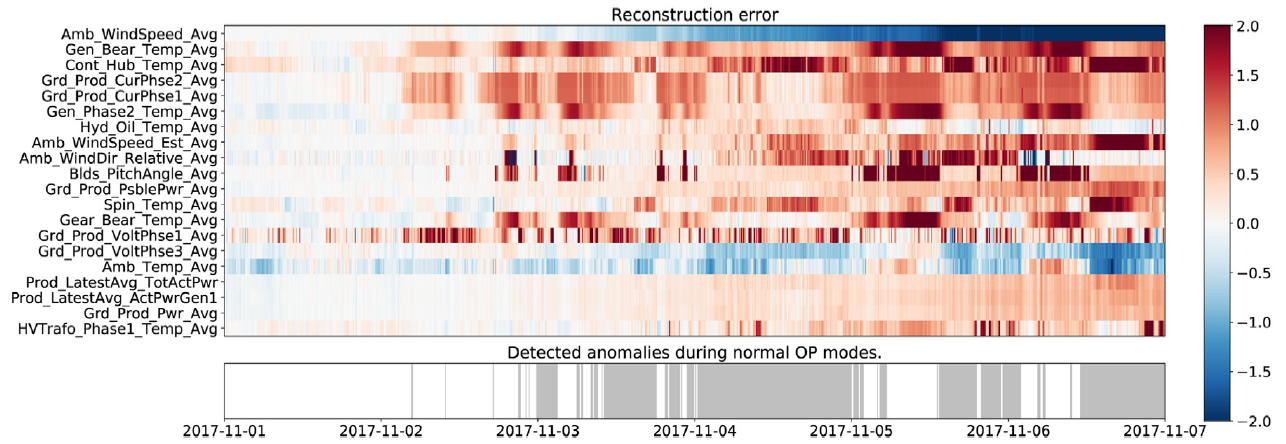
\includegraphics[width=\textwidth]{Figures/Chapter03/Fig.03.60_Heatmap.png}
	\caption{Heat map of the scaled reconstruction error for the prediction period with added wind speed sensor error \parencite{roelofs2021autoencoder}}
	\label{fig03.60}
\end{figure}

\begin{figure}[h]
	\centering
	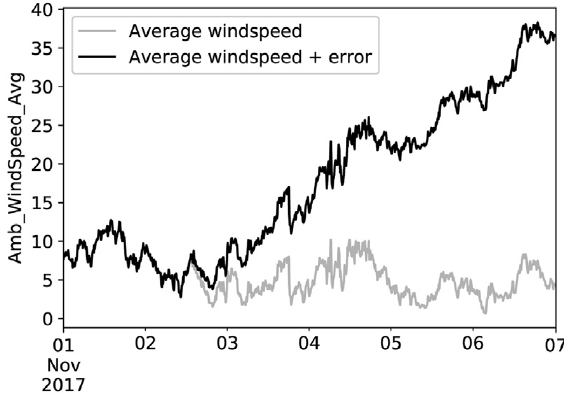
\includegraphics[width=0.5\textwidth]{Figures/Chapter03/Fig.03.61_simErr.png}
	\caption{Simulated error added to good condition data \parencite{roelofs2021autoencoder}}
	\label{fig03.61}
\end{figure}

However, this analysis cannot isolate the root cause of the anomaly because the fully connected structure of neural network allows the error to be propagated and affect all outputs (Fig. \ref{fig03.62}).

\begin{figure}[h!]
	\centering
	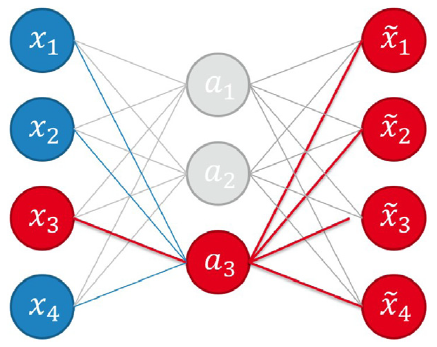
\includegraphics[width=0.35\textwidth]{Figures/Chapter03/Fig.03.62_Err.png}
	\caption{Error is propagated through the network \parencite{roelofs2021autoencoder}}
	\label{fig03.62}
\end{figure}
%\caption{Error is propagated through the network and affect all outputs \parencite{roelofs2021autoencoder}}

To solve this problem, they propose and implement the ARCANA (Anomaly Root Cause Analysis) algorithm to find which inputs contributes to the anomaly detected by the AutoEncoder. Fig. \ref{fig03.63} shows that the ARCANA algorithm can recognize which abnormal signal can be the root cause of the anomaly.

\begin{figure}[h]
	\centering
	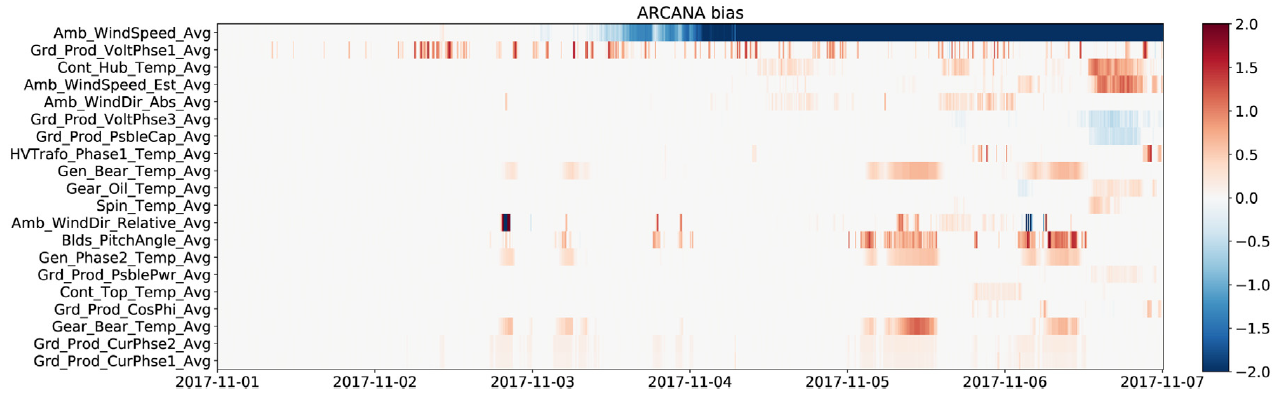
\includegraphics[width=\textwidth]{Figures/Chapter03/Fig.03.63_Heatmap_after.png}
	\caption{Heat map after applied the ARCANA algorithm \parencite{roelofs2021autoencoder}}
	\label{fig03.63}
\end{figure}

Although explainable AI is not in the scope of this work, from their result, we know that analyzing Reconstruction Error of each signal cannot help to discover the root cause of the anomaly. Therefore, this function will not be implemented in the software.

\hspace{1cm}\\
\textbf{Using an autoencoder in the design of an anomaly detector for smart manufacturing} \parencite{alfeo2020using}

The Anomaly Detection solution by Alfeo et al. aims at supporting smart manufacturing operators with no data science background . The development of anomaly detection solutions in real-world manufacturing demands a trade-off between system management cost and detection accuracy. It depends on the anomaly threshold which distinguishes normal data and anomalous data. Restrictive thresholds may increase the false negatives, while loose thresholds result in many false positives. In the machine learning pipeline with the involvement of three roles (Data Engineer, Data Scientist and Business Expert), the Data Scientist is in charge of the Anomaly Threshold setup (Fig. \ref{fig03.64}).

\begin{figure}[h!]
	\centering
	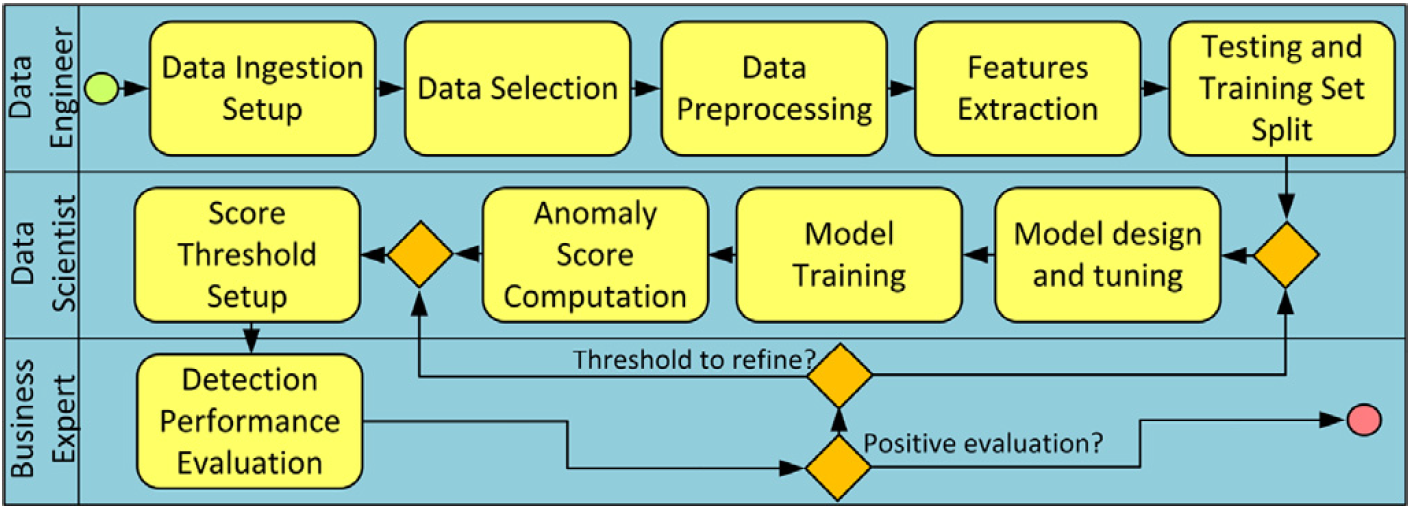
\includegraphics[width=0.9\textwidth]{Figures/Chapter03/Fig.03.64_pipeline.png}
	\caption{Anomaly detection pipeline \parencite{alfeo2020using}}
	\label{fig03.64}
\end{figure}

In order to improve process performance, they develop a Discriminator that can adjust the anomaly score threshold automatically using heuristic-based algorithms (Fig. \ref{fig03.65}).

\begin{figure}[h!]
	\centering
	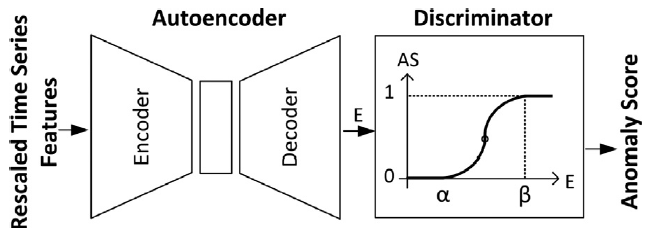
\includegraphics[width=0.65\textwidth]{Figures/Chapter03/Fig.03.65_threshold.png}
	\caption{Discriminator for Anomaly Score \parencite{alfeo2020using}}
	\label{fig03.65}
\end{figure}

Their case study is the washing process of industry laundry. They compare their results with Isolation Forest, the current best-in-class Anomaly Detection algorithm.

Although automating the Anomaly Threshold is not in the scope of this work, their Anomaly Detection pipeline makes clear the user roles and the necessary collaboration between them for anomaly detection, which is rarely discussed in researches of this topic. 

Their pipeline also inspires us to define user roles (Machine Operator, Machine Expert) of the Predictive Maintenance software so that the AutoEncoder can be trained and re-trained efficiently with right data. The Data Scientist role in the organization also inspires us to create a open mechanism so that Data Scientist users can replace our built-in AutoEncoder model by their own models.

\subsection{Conclusion}

In conclusion, after reviewing several state-of-the-art studies of Predictive Maintenance, especially studies of Anomaly Detection, the AutoEncoder-based Anomaly Detection method is chosen for the proposed Predictive Maintenance system implemented in this work.

The Convolutional Deep AutoEncoder (CDAE) implemented by Convolutional Neural Network (CNN) is chosen as the built-in AutoEncoder for monitoring data Reconstruction Error, although it is open for Data Scientist users to import their own AutoEncoder models.

The predictive model should be as general and scalable as possible, not based on characteristics of specific dataset or machines, requiring minimum detailed knowledge of monitored machines, although machine expertise will be helpful. This is the objective and also the ambition of this work.
